\chapter{APPROXIMATION METHODS}
Perturbation theory is based on the assumption that the problem we wish to solve is, in some sense, only slightly different from a problem that can be solved exactly. In the case where the deviation between the two problems is small, perturbation theory is suitable for calculating the contribution associated with this deviation; this contribution is then added as a correction to the energy and the wave function of the exactly solvable Hamiltonian. So perturbation theory builds on the known exact solutions to obtain approximate solutions.\\
What about those systems whose Hamiltonians cannot be reduced to an exactly solvable part plus a small correction. For these, we may consider the variational method or the WKB approximation. The variational method is particularly useful in estimating the energy eigenvalues of the ground state and the first few excited states of a system for which one has only a qualitative idea about the form of the wave function.\\
The WKB method is useful for finding the energy eigenvalues and wave functions of systems for which the classical limit is valid. 
\section{Time Independent Perturbation Theory}
This method is most suitable when $\hat{H}$ is very close to a Hamiltonian $H_{0}$ that can be solved exactly. In this case, $\hat{H}$ can be split into two time-independent parts
$$
\hat{H}=\hat{H}_{0}+\hat{H}_{p},
$$
where $\hat{H}_{p}$ is very small compared to $\hat{H}_{0}\left(\hat{H}_{0}\right.$ is known as the Hamiltonian of the unperturbed system). As a result, $\hat{H}_{p}$ is called the perturbation, for its effects on the energy spectrum and eigenfunctions will be small; such perturbation is encountered, for instance, in systems subject to weak electric or magnetic fields. We can make this idea more explicit by writing $\hat{H}_{p}$ in terms of a dimensionless real parameter $\lambda$ which is very small compared to 1 :
$$
\hat{H}_{p}=\lambda \hat{W} \quad(\lambda \ll 1) .
$$
Thus the eigenvalue problem becomes
$$
\left(\hat{H}_{0}+\lambda \hat{W}\right)\left|\psi_{n}\right\rangle=E_{n}\left|\psi_{n}\right\rangle .
$$
In what follows we are going to consider two separate cases depending on whether the exact solutions of $\hat{H}_{0}$ are nondegenerate or degenerate. Each of these two cases requires its own approximation scheme.
\subsection{Nondegenerate Perturbation Theory}
In this section we limit our study to the case where $\hat{H}_{0}$ has no degenerate eigenvalues; that is, for every energy $E_{n}^{(0)}$ there corresponds only one eigenstate $\left|\phi_{n}\right\rangle:$
$$
\hat{H}_{0}\left|\phi_{n}\right\rangle=E_{n}^{(0)}\left|\phi_{n}\right\rangle,
$$
where the exact eigenvalues $E_{n}^{(0)}$ and exact eigenfunctions $\left|\phi_{n}\right\rangle$ are known.\\

The main idea of perturbation theory consists in assuming that the perturbed eigenvalues and eigenstates can both be expanded in power series in the parameter $\lambda$ :
$$
\begin{aligned}
E_{n} &=E_{n}^{(0)}+\lambda E_{n}^{(1)}+\lambda^{2} E_{n}^{(2)}+\cdots \\
\left|\psi_{n}\right\rangle &=\left|\phi_{n}\right\rangle+\lambda\left|\psi_{n}^{(1)}\right\rangle+\lambda^{2}\left|\psi_{n}^{(2)}\right\rangle+\cdots
\end{aligned}
$$

The job of perturbation theory reduces then to the calculation of $E_{n}^{(1)}, E_{n}^{(2)}, \ldots$ and $\left|\psi_{n}^{(1)}\right\rangle$, $\left|\psi_{n}^{(2)}\right\rangle, \ldots .$ In this section we shall be concerned only with the determination of $E_{n}^{(1)}, E_{n}^{(2)}$, and $\left|\psi_{n}^{(1)}\right\rangle .$ Assuming that the unperturbed states $\left|\phi_{n}\right\rangle$ are nondegenerate, and substituting the power series expansion of $E_{n}$ and $\left|\psi_{n}\right\rangle $ in $
\left(\hat{H}_{0}+\lambda \hat{W}\right)\left|\psi_{n}\right\rangle=E_{n}\left|\psi_{n}\right\rangle .
$ we obtain
$$
\begin{aligned}
&\left(\hat{H}_{0}+\lambda \hat{W}\right)\left(\left|\phi_{n}\right\rangle+\lambda\left|\psi_{n}^{(1)}\right\rangle+\lambda^{2}\left|\psi_{n}^{(2)}\right\rangle+\cdots\right) \\
&\quad=\left(E_{n}^{(0)}+\lambda E_{n}^{(1)}+\lambda^{2} E_{n}^{(2)}+\cdots\right)\left(\left|\phi_{n}\right\rangle+\lambda\left|\psi_{n}^{(1)}\right\rangle+\lambda^{2}\left|\psi_{n}^{(2)}\right\rangle+\cdots\right)
\end{aligned}
$$
The coefficients of successive powers of $\lambda$ on both sides of this equation must be equal. Equating the coefficients of the first three powers of $\lambda$, we obtain these results:
	$$
	\begin{aligned}
	\text{- Zero order in $\lambda$ :}&\\
	&\hat{H}_{0}\left|\phi_{n}\right\rangle=E_{n}^{(0)}\left|\phi_{n}\right\rangle\\
	\text{- First order in $\lambda:$}&\\
	&\hat{H}_{0}\left|\psi_{n}^{(1)}\right\rangle+\hat{W}\left|\phi_{n}\right\rangle=E_{n}^{(0)}\left|\psi_{n}^{(1)}\right\rangle+E_{n}^{(1)}\left|\phi_{n}\right\rangle\\
	\text{- Second order in $\lambda$ :}&\\
&\hat{H}_{0}\left|\psi_{n}^{(2)}\right\rangle+\hat{W}\left|\psi_{n}^{(1)}\right\rangle=E_{n}^{(0)}\left|\psi_{n}^{(2)}\right\rangle+E_{n}^{(1)}\left|\psi_{n}^{(1)}\right\rangle+E_{n}^{(2)}\left|\phi_{n}\right\rangle
\end{aligned}
$$

We now proceed to determine the eigenvalues $E_{n}^{(1)}, E_{n}^{(2)}$ and the eigenvector $\left|\psi_{n}^{(1)}\right\rangle$  For this, we need to specify how the states $\left|\phi_{n}\right\rangle$ and $\left|\psi_{n}\right\rangle$ overlap. Since $\left|\psi_{n}\right\rangle$ is considered not to be very different from $\left|\phi_{n}\right\rangle$, we have $\left\langle\phi_{n} \mid \psi_{n}\right\rangle \simeq 1 .$ We can, however. normalize $\left|\psi_{n}\right\rangle$ so that its overlap with $\left|\phi_{n}\right\rangle$ is exactly equal to one:
\begin{align*}
\left\langle\phi_{n} \mid \psi_{n}\right\rangle&=1 .\\
\text{Substituting power series expansion of }&\text{$\left|\psi_{n}\right\rangle $ ine above equation we get}\\
\lambda\left\langle\phi_{n} \mid \psi_{n}^{(1)}\right\rangle+\lambda^{2}\left\langle\phi_{n} \mid \psi_{n}^{(2)}\right\rangle+\cdots&=0\\
\text{hence the coefficients of the various powers of }&\text{$\lambda$ must vanish separately:}\\
\left\langle\phi_{n} \mid \psi_{n}^{(1)}\right\rangle=\left\langle\phi_{n} \mid \psi_{n}^{(2)}\right\rangle=\cdots&=0 
\end{align*}
\subsubsection{First Order Correction}
\begin{align*}
E_{n}^{(1)}&=\left\langle\phi_{n}|\hat{W}| \phi_{n}\right\rangle\\
\text{Energy of first}&\text{ order pertubration}\\
E_{n}&=E_{n}^{(0)}+\left\langle\phi_{n}\left|\hat{H}_{p}\right| \phi_{n}\right\rangle\\
\text{First order correction }&\text{of eigen vector}\\
\left|\psi_{n}^{(1)}\right\rangle&=\sum_{m \neq n} \frac{\left\langle\phi_{m}|\hat{W}| \phi_{n}\right\rangle}{E_{n}^{(0)}-E_{m}^{(0)}}\left|\phi_{m}\right\rangle\\
\text{The eigenfunction $\left|\psi_{n}\right\rangle$ of $\hat{H}$ to}&\text{ first order in $\lambda \hat{W}$ can then be obtained as}\\
\left|\psi_{n}\right\rangle&=\left|\phi_{n}\right\rangle+\sum_{m \neq n} \frac{\left\langle\phi_{m}\left|\hat{H}_{p}\right| \phi_{n}\right\rangle}{E_{n}^{(0)}-E_{m}^{(0)}}\left|\phi_{m}\right\rangle
\end{align*}
\subsubsection{Second Order Correction}
\begin{align*}
E_{n}^{(2)}&=\left\langle\phi_{n}|\hat{W}| \psi_{n}^{(1)}\right\rangle\\
\text{which can  be}&\text{ written as}\\
E_{n}^{(2)}&=\sum_{m \neq n} \frac{\left|\left\langle\phi_{m}|\hat{W}| \phi_{n}\right\rangle\right|^{2}}{E_{n}^{(0)}-E_{m}^{(0)}}\\
\text{ The eigenenergy}&\text{ to second order in $ \hat{H}_{p}$ is obtained as }\\
E_{n}&=E_{n}^{(0)}+\left\langle\phi_{n}\left|\hat{H}_{p}\right| \phi_{n}\right\rangle+\sum_{m \neq n} \frac{\left|\left\langle\phi_{m}\left|\hat{H}_{p}\right| \phi_{n}\right\rangle\right|^{2}}{E_{n}^{(0)}-E_{m}^{(0)}}+\cdots .
\end{align*}






\subsubsection{Application}
\subsubsection{Stark Effect(n=1-Non Degenerate Case)}

 The effect that an external electric field has on the energy levels of an atom is called the Stark effect. In the absence of an electric field, the (unperturbed) Hamiltonian of the hydrogen atom (in CGS units) is:
$$
\hat{H}_{0}=\frac{\hat{\vec{p}}^{2}}{2 \mu}-\frac{e^{2}}{r} .
$$
The eigenfunctions of this Hamiltonian, $\psi_{n l m}(\vec{r})$, are given by
$$
\langle r \theta \varphi \mid n l m\rangle=\psi_{n l m}(r, \theta, \varphi)=R_{n l}(r) Y_{l m}(\theta, \varphi) .
$$
When the electric field is turned on, the interaction between the atom and the field generates a term $\hat{H}_{p}=e \overrightarrow{\mathcal{E}} \cdot \vec{r}=e \mathcal{E} \hat{Z}$ that needs to be added to $\hat{H}_{0}$.

Since the excited states of the hydrogen atom are degenerate while the ground state is not, nondegenerate perturbation theory applies only to the ground state, $\psi_{100}(\vec{r})$. Ignoring the spin degrees of freedom, the energy of this system to second-order perturbation is given as follows
	$$
	\begin{aligned}
	&E_{100}=E_{100}^{(0)}+e \mathcal{E}\langle 100|\hat{Z}| 100\rangle+e^{2} \mathcal{E}^{2} \sum_{n l m \neq 100} \frac{|\langle n l m|\hat{Z}| 100\rangle|^{2}}{E_{100}^{(0)}-E_{n l m}^{(0)}}\\
	\text{The term}&\\
	&\langle 100|\hat{Z}| 100\rangle=\int\left|\psi_{100}(\vec{r})\right|^{2} z d^{3} r
\end{aligned}
$$
is zero, since $\hat{Z}$ is odd under parity and $\psi_{100}(\vec{r})$ has a definite parity. This means that there can be no correction term to the energy which is proportional to the electric field and hence there is no linear Stark effect. The underlying physics behind this is that when the hydrogen atom is in its ground state, it has no permanent electric dipole moment. We are left then with only a quadratic dependence of the energy  on the electric field. This is called the quadratic Stark effect. This correction, which is known as the energy shift $\Delta E$, is given by
$$
\Delta E=e^{2} \mathcal{E}^{2} \sum_{n l m \neq 100} \frac{|\langle n l m|\hat{Z}| 100\rangle|^{2}}{E_{100}^{(0)}-E_{n l m}^{(0)}}
$$
\subsection{Degenerate Perturbation Theory}
 We now apply perturbation theory to determine the energy spectrum and the states of a system whose unperturbed Hamiltonian $\hat{H}_{0}$ is degenerate:
$$
\hat{H}\left|\psi_{n}\right\rangle=\left(\hat{H}_{0}+\hat{H}_{p}\right)\left|\psi_{n}\right\rangle=E_{n}\left|\psi_{n}\right\rangle .
$$
If, for instance, the level of energy $E_{n}^{(0)}$ is $f$-fold degenerate (i.e., there exists a set of $f$ different eigenstates $\left|\phi_{n_{\alpha}}\right\rangle$, where $\alpha=1,2, \ldots, f$, that correspond to the same eigenenergy $\left.E_{n}^{(0)}\right)$, we have
$$
\hat{H}_{0}\left|\phi_{n_{\alpha}}\right\rangle=E_{n}^{(0)}\left|\phi_{n_{\alpha}}\right\rangle \quad(\alpha=1,2, \ldots, f),
$$
where $\alpha$ stands for one or more quantum numbers; the energy eigenvalues $E_{n}^{(0)}$ are independent of $\alpha$.

In the zeroth-order approximation we can write the eigenfunction $\left|\psi_{n}\right\rangle$ as a linear combination in terms of $\left|\phi_{n_{a}}\right\rangle$ :
$$
\left|\psi_{n}\right\rangle=\sum_{\alpha=1}^{f} a_{\alpha}\left|\phi_{n_{\alpha}}\right\rangle .
$$
Considering the states $\left|\phi_{n_{a}}\right\rangle$ to be orthonormal with respect to the label $\alpha$ (i.e., $\left\langle\phi_{n_{a}} \mid \phi_{n_{\beta}}\right\rangle=$ $\left.\delta_{a, \beta}\right)$ and $\left|\psi_{n}\right\rangle$ to be normalized, $\left\langle\psi_{n} \mid \psi_{n}\right\rangle=1$, we can ascertain that the coefficients $a_{\alpha}$ obey the relation
$$
\left\langle\psi_{n} \mid \psi_{n}\right\rangle=\sum_{\alpha, \beta} a_{\alpha}^{*} a_{\beta} \delta_{\alpha, \beta}=\sum_{\alpha=1}^{f}\left|a_{\alpha}\right|^{2}=1 .
$$
In what follows we are going to show how to determine these coefficients and the first-order corrections to the energy. For this, let us substitute $
\left|\psi_{n}\right\rangle=\sum_{\alpha=1}^{f} a_{\alpha}\left|\phi_{n_{\alpha}}\right\rangle .
$ and $
\hat{H}_{0}\left|\phi_{n_{\alpha}}\right\rangle=E_{n}^{(0)}\left|\phi_{n_{\alpha}}\right\rangle \quad(\alpha=1,2, \ldots, f),
$ into eigen value equation(perturbed) we will get
$$
\sum_{a}\left[E_{n}^{(0)}\left|\phi_{n_{u}}\right\rangle+\hat{H}_{p}\left|\phi_{n_{u}}\right\rangle\right] a_{\alpha}=E_{n} \sum_{\alpha} a_{a}\left|\phi_{n_{a}}\right\rangle
$$
The multiplication of both sides of this equation by $\left\langle\phi_{n_{\beta}}\right|$ leads to
$$
\sum_{u} a_{u}\left[E_{n}^{(0)} \delta_{u, \beta}+\left\langle\phi_{n_{j}}\left|\hat{H}_{p}\right| \phi_{n_{a}}\right\rangle\right]=E_{n} \sum_{\alpha} a_{a} \delta_{\alpha, \beta}
$$
or 10
$$
a_{\beta} E_{n}=a_{\beta} E_{n}^{(0)}+\sum_{\alpha=1}^{f} a_{u}\left\langle\phi_{n_{n}}\left|\hat{H}_{p}\right| \phi_{n_{a}}\right\rangle,
$$
where we have used $\left\langle\phi_{n \beta} \mid \phi_{n_{a}}\right\rangle=\delta_{\beta, a}$. We can rewrite the above equation as 
$$
\sum_{a=1}^{f}\left(\hat{H}_{p_{\beta a}}-E_{n}^{(1)} \delta_{\alpha, \beta}\right) a_{\alpha}=0 \quad(\beta=1,2, \ldots, f),
$$
with $\hat{H}_{p_{\beta a}}=\left\langle\phi_{n_{\beta}}\left|\hat{H}_{p}\right| \phi_{n_{u}}\right\rangle$ and $E_{n}^{(1)}=E_{n}-E_{n}^{(0)}$. This is a system of $f$ homogeneous linear equations for the coefficients $a_{\alpha}$. These coefficients are nonvanishing only when the determinant $\left|\hat{H}_{p_{a \beta}}-E_{n}^{(1)} \delta_{\alpha, \beta}\right|$ is zero:
$$\left|\begin{array}{ccccc}
	\hat{H}_{p_{11}}-E_{n}^{(1)} & \hat{H}_{p_{12}} & \hat{H}_{p_{13}} & \cdots & \hat{H}_{p_{1 /}} \\
	\hat{H}_{p_{21}} & \hat{H}_{p_{22}}-E_{n}^{(1)} & \hat{H}_{p_{23}} & \cdots & \hat{H}_{p_{2} f} \\
	\vdots & \vdots & \vdots & \ddots & \vdots \\
	\hat{H}_{p_{f 1}} & \hat{H}_{p_{f 2}} & \hat{H}_{p_{f 3}} & \cdots & \hat{H}_{p_{f f}}-E_{n}^{(1)}
\end{array}\right|=0$$
 In summary, to determine the eigenvalues to first-order and the eigenstates to zeroth order for an $f$-fold degenerate level from perturbation theory, we proceed as follows:
 \begin{itemize}
 	\item First, for each $f$-fold degenerate level, determine the $f \times f$ matrix of the perturbation $\hat{H}_{p}$ :
 	$$H_{p}=\left(\begin{array}{cccc}
 		\hat{H}_{p_{11}} & \hat{H}_{p_{12}} & \cdots & \hat{H}_{p_{1 f}} \\
 		\hat{H}_{p_{21}} & \hat{H}_{p_{22}} & \cdots & \hat{H}_{p_{2 f}} \\
 		\vdots & \vdots & \ddots & \vdots \\
 		\hat{H}_{p_{f 1}} & \hat{H}_{p_{f 2}} & \cdots & \hat{H}_{p_{f \prime}}
 	\end{array}\right)$$
 	\item Second, diagonalize this matrix and find the $f$ eigenvalues $E_{n_{a}}^{(1)}(\alpha=1,2, \ldots, f)$ and their corresponding eigenvectors\\
 	$$a_{\alpha}=\left(\begin{array}{c}
 		a_{\alpha_{1}} \\
 		a_{\alpha_{2}} \\
 		\vdots \\
 		a_{a_{f}}
 	\end{array}\right) \quad(\alpha=1,2, \ldots, f)$$
 	\item Finally, the energy eigenvalues are given to first order by
 	$$
 	E_{n_{a}}=E_{n}^{(0)}+E_{n_{a}}^{(1)} \quad(\alpha=1,2, \ldots, f)
 	$$
 	and the corresponding eigenvectors are given to zero order by
 	$$
 	\left|\psi_{n_{a}}\right\rangle=\sum_{\beta=1}^{f} a_{\alpha \beta}\left|\phi_{n_{\beta}}\right\rangle
 	$$
 \end{itemize}

\subsubsection{Application}
\textbf{Stark Effect N=2 Degenerate States}\\
In the absence of any external electric field, the first excited state (i.e., $n=2$ ) is fourfold degenerate: the states $|n l m\rangle=|200\rangle,|210\rangle,|211\rangle$, and $|21-1\rangle$ have the same energy $E_{2}=-R_{y} / 4$, where $R_{y}=\mu e^{4} /\left(2 \hbar^{2}\right)=13.6 \mathrm{eV}$ is the Rydberg constant.

When the external electric field is turned on, some energy levels will split. The energy due to the interaction between the dipole moment of the electron $(\vec{d}=-e \vec{r})$ and the external electric field $(\overrightarrow{\mathcal{E}}=\overrightarrow{\mathcal{E}} \vec{k})$ is given by
$$
\hat{H}_{p}=-\vec{d} \cdot \overrightarrow{\mathcal{E}}=e \vec{r} \cdot \overrightarrow{\mathcal{E}}=e \mathcal{E} \hat{Z}
$$
To calculate the eigenenergies, we need to determine and then diagonalize the $4 \times 4$ matrix elements of $\hat{H}_{p}:\left\langle 2 l^{\prime} m^{\prime}\left|\hat{H}_{p}\right| 2 l m\right\rangle=e \mathcal{E}\left\langle 2 l^{\prime} m^{\prime}|\hat{Z}| 2 l m\right\rangle .$ The matrix elements $\left\langle 2 l^{\prime} m^{\prime}|\hat{Z}|\right.$ $2 l m)$ can be calculated more simply by using the relevant selection rules and symmetries. First, since $\hat{Z}$ does not depend on the azimuthal angle $\varphi, z=r \cos \theta$, the elements $\left\langle 2 l^{\prime} m^{\prime}|\hat{Z}| 2 l m\right\rangle$ are nonzero only if $m^{\prime}=m$. Second, as $Z$ is odd, the states $\left|2 l^{\prime} m^{\prime}\right\rangle$ and $|2 l m\rangle$ must have opposite parities so that $\left\langle 2 l^{\prime} m^{\prime}|\hat{Z}| 2 l m\right\rangle$ does not vanish. Therefore, the only nonvanishing matrix elements are those that couple the $2 \mathrm{~s}$ and $2 \mathrm{p}$ states (with $m=0$ ); that is, between | 200) and $|210\rangle$. In this case we have\\
$$\begin{aligned}
	\langle 200|\hat{Z}| 210\rangle &=\int_{0}^{\infty} R_{20}^{*}(r) R_{21}(r) r^{2} d r \int Y_{00}^{*}(\Omega) z Y_{10}(\Omega) d \Omega \\
	&=\sqrt{\frac{4 \pi}{3}} \int_{0}^{\infty} R_{20}(r) R_{21}(r) r^{3} d r \int Y_{00}^{*}(\Omega) Y_{10}^{2}(\Omega) d \Omega \\
	&=-3 a_{0},
\end{aligned}$$
since $z=r \cos \theta=\sqrt{4 \pi / 3} r Y_{10}(\Omega),\langle\vec{r} \mid 200\rangle=R_{20}(r) Y_{00}(\Omega),\langle\vec{r} \mid 210\rangle=R_{21}(r) Y_{10}(\Omega)$, and $d \Omega=\sin \theta d \theta d \varphi ; a_{0}=\hbar^{2} /\left(\mu e^{2}\right)$ is the Bohr radius. Using the notations $|1\rangle=|200\rangle$, $|2\rangle=|21|\rangle,|3\rangle=|210\rangle$, and $|4\rangle=|21-1\rangle$, we can write the matrix of $H_{p}$ as
$$
H_{p}=\left(\begin{array}{ccccc}
\left\langle 1\left|\hat{H}_{p}\right| 1\right\rangle & \left\langle 1\left|\hat{H}_{p}\right| 2\right\rangle & \left\langle 1\left|\hat{H}_{p}\right| 3\right\rangle & \left\langle 1\left|\hat{H}_{p}\right| 4\right\rangle \\
\left\langle 2\left|\hat{H}_{p}\right| 1\right\rangle & \left\langle 2\left|\hat{H}_{p}\right| 2\right\rangle & \left\langle 2\left|\hat{H}_{p}\right| 3\right\rangle & \left\langle 2\left|\hat{H}_{p}\right| 4\right\rangle \\
\left\langle 3\left|\hat{H}_{p}\right| 1\right\rangle & \left\langle 3\left|\hat{H}_{p}\right| 2\right\rangle & \left\langle 3\left|\hat{H}_{p}\right| 3\right\rangle & \left\langle 3\left|\hat{H}_{p}\right| 4\right\rangle \\
\left\langle 4\left|\hat{H}_{p}\right| 1\right\rangle & \left\langle 4\left|\hat{H}_{p}\right| 2\right\rangle & \left\langle 4\left|\hat{H}_{p}\right| 3\right\rangle & \left\langle 4\left|\hat{H}_{p}\right| 4\right\rangle
\end{array}\right)
$$
$$H_{p}=-3 e \mathcal{E} a_{0}\left(\begin{array}{cccc}
	0 & 0 & 1 & 0 \\
	0 & 0 & 0 & 0 \\
	1 & 0 & 0 & 0 \\
	0 & 0 & 0 & 0
\end{array}\right)$$

The diagonalization of this matrix leads to the following eigenvalues:
$$
E_{2}^{(1)},=-3 e \mathcal{E} a_{0}, \quad E_{2}^{(1)}{ }_{2}=E_{2}^{(1)}{ }_{3}=0, \quad E_{2{ }^{(1)}}{ }_{4}=3 e \mathcal{E} a_{0} .
$$
Thus, the energy levels of the $n=2$ states are given to first order by
$$
E_{2_{1}}=-\frac{R_{y}}{4}-3 e \mathcal{E} a_{0}, \quad E_{2_{2}}=E_{2_{3}}=-\frac{R_{y}}{4}, \quad E_{2_{4}}=-\frac{R_{y}}{4}+3 e \mathcal{E} a_{0} .
$$
The corresponding eigenvectors to zeroth order are
$$
\begin{aligned}
&\left|\psi_{2}\right\rangle_{1}=\frac{1}{\sqrt{2}}(|200\rangle+|210\rangle), \quad\left|\psi_{2}\right\rangle_{2}=|211\rangle, \\
&\left|\psi_{2}\right\rangle_{3}=|21-1\rangle, \quad\left|\psi_{2}\right\rangle_{4}=\frac{1}{\sqrt{2}}(|200\rangle-|210\rangle) .
\end{aligned}
$$
This perturbation has only partially removed the degeneracy of the $n=2$ level; the states $|211\rangle$ and $|21-1\rangle$ still have the same energy $E_{3}=E_{4}=-R_{y} / 4$.

\subsection{Spin Orbit Coupling}
One of the most useful applications of perturbation theory is to calculate the energy corrections for the hydrogen atom, notably the corrections due to the fine structure. The fine structure is in turn due to two effects: spin-orbit coupling and the relativistic correction. Let us look at these corrections separately.\\
\par The spin-orbit coupling in hydrogen arises from the interaction between the electron's spin magnetic moment, $\vec{\mu}_{S}=-e \vec{S} /\left(m_{e} c\right)$, and the proton's orbital magnetic field $\vec{B}$.

The origin of the magnetic field experienced by the electron moving at $\vec{v}$ in a circular orbit around the proton can be explained classically as follows. The electron, within its rest frame. sees the proton moving at $-\vec{v}$ in a circular orbit around it . From classical electrodynamics, the magnetic field experienced by the electron is
	$$
	\begin{aligned}
	\vec{B}&=-\frac{1}{c} \vec{v} \times \vec{E}=-\frac{1}{m_{e} c} \vec{p} \times \vec{E}=\frac{1}{m_{e} c} \vec{E} \times \vec{p},\\
	\text{But }\quad\vec{E}(\vec{r})&=-\vec{\nabla} \phi(r)=\frac{1}{e} \vec{\nabla} V(r)=\frac{1}{e} \frac{\vec{r}}{r} \frac{d V}{d r} \\
	\text{Then B is }\quad\vec{B}&=\frac{1}{m_{e} c} \vec{E} \times \vec{p}=\frac{1}{e m_{e} c} \frac{1}{r} \frac{d V}{d r} \vec{r} \times \vec{p}=\frac{1}{e m_{e} c} \frac{1}{r} \frac{d V}{d r} \vec{L}\\
\text{	where }\quad\vec{L}&=\vec{r} \times \vec{p}\text{ is the orbital angular momentum of the electron.}
\end{aligned}
$$
where $\vec{L}=\vec{r} \times \vec{p}$ is the orbital angular momentum of the electron.
The interaction of the electron's spin dipole moment $\vec{\mu}_{S}$ with the orbital magnetic field $\vec{B}$ of the nucleus gives rise to the following interaction energy:
	$$
	\begin{aligned}
	\hat{H}_{S O}&=-\vec{\mu}_{S} \cdot \vec{B}=\frac{e}{m_{e} c} \vec{S} \cdot \vec{B}=\frac{1}{m_{e}^{2} c^{2}} \frac{1}{r} \frac{d V}{d r} \vec{S} \cdot \vec{L}\\
	\text{ This energy turns out }&\text{to be twice the observed spin-orbit interaction.Therefore}\\
	\hat{H}_{S O}&=\frac{1}{2 m_{e}^{2} c^{2}} \frac{1}{r} \frac{d V}{d r} \vec{S} \cdot \vec{L}\\
	\text{ The corresponding }&\text{quantum mechanical expression}\\
\hat{H}_{S O}&=\frac{1}{2 m_{e}^{2} c^{2}} \frac{1}{r} \frac{d \hat{V}}{d r} \hat{S} \cdot \hat{\vec{L}}\\
\text{	For a hydrogen's electron, $V(r)$}&=\text{	$-e^{2} / r$ and $d V / d r=e^{2} / r^{2}$.}\\
	\hat{H}_{S O}&=\frac{e^{2}}{2 m_{e}^{2} c^{2}} \frac{1}{r^{3}} \hat{S} \cdot \hat{L}\\
\text{	We can now use perturbation theory }&\text{to calculate the contribution of the spin-orbit interaction in a hydrogen atom:}\\
	\hat{H}&=\frac{\hat{\vec{p}}^{2}}{2 m_{e}}-\frac{e^{2}}{r}+\frac{e^{2}}{2 m_{e}^{2} c^{2} r^{3}} \hat{\vec{S}} \cdot \hat{\vec{L}}=\hat{H}_{0}+\hat{H}_{S O}
\end{aligned}
$$
where $\hat{H}_{0}$ is the unperturbed Hamiltonian and $\hat{H}_{S O}$ is the perturbation. To apply perturbation theory, we need to specify the unperturbed states-the eigenstates of $\hat{H}_{0 .}$ Since the spin of the hydrogen's electron is taken into account, the total wave function of $\hat{H}_{0}$ consists of a direct product of two parts: a spatial part and a spin part. \\
The eigen state is 
	$$
	\begin{aligned}
	\Psi_{n, l, j=l \pm \frac{1}{2}, m}&=R_{n l}(r)\left[\sqrt{\frac{l \mp m+\frac{1}{2}}{2 l+1}} Y_{l, m+\frac{1}{2}}\left|\frac{1}{2},-\frac{1}{2}\right\rangle \pm \sqrt{\frac{l \pm m+\frac{1}{2}}{2 l+1}} Y_{l, m-\frac{1}{2}}\left|\frac{1}{2}, \frac{1}{2}\right\rangle\right]\\
\text{	The corresponding }&\text{eigenvalues are given by}\\
	\langle n l j m|\hat{\vec{L}} \cdot \hat{\vec{S}}| n l j m\rangle&=\frac{\hbar^{2}}{2}\left[j(j+1)-l(l+1)-\frac{3}{4}\right]\\
	\text { since } \hat{\vec{S}} \cdot \hat{\vec{L}}&=\frac{1}{2}\left[\hat{J}^{2}-\hat{L}^{2}-\hat{S}^{2}\right]\\
	\text{The eigenvalues of total }&\text{Hamiltonian H are then given to first-order correction by}
\end{aligned}
$$
$$
E_{n l j}=E_{n}^{(0)}+\left\langle n l j m_{j}\left|\hat{H}_{S O}\right| n l j m_{j}\right\rangle=-\frac{e^{2}}{2 a_{0}} \frac{1}{n^{2}}+E_{S O}^{(1)}
$$
where $E_{n}^{(0)}=-e^{2} /\left(2 a_{0} n^{2}\right)=-\left(13.6 / n^{2}\right) \mathrm{eV}$ are the energy levels of hydrogen and $E_{S O}^{(1)}$ is the energy due to spin-orbit interaction:
	$$
	\begin{aligned}
	E_{S O}^{(1)}=\left\langle n l j m_{j}\left|\hat{H}_{S O}\right| n l j m_{j}\right\rangle&=\frac{e^{2} \hbar^{2}}{4 m_{e}^{2} c^{2}}\left[j(j+1)-l(l+1)-\frac{3}{4}\right]\left\langle n l\left|\frac{1}{r^{3}}\right| n l\right\rangle\\
	\left\langle n l\left|\frac{1}{r^{3}}\right| n l\right\rangle&=\frac{2}{n^{3} l(l+1)(2 l+1) a_{0}^{3}}\\
	E_{S O}^{(1)}&=\frac{e^{2} \hbar^{2}}{2 m_{e}^{2} c^{2}}\left[\frac{j(j+1)-l(l+1)-\frac{3}{4}}{n^{3} l(l+1)(2 l+1) a_{0}^{3}}\right]\\
		&=\left(\frac{e^{2}}{2 a_{0}} \frac{1}{n^{2}}\right)\left(\frac{\hbar}{m_{e} c a_{0}}\right)^{2} \frac{1}{n}\left[\frac{j(j+1)-l(l+1)-\frac{3}{4}}{l(l+1)(2 l+1)}\right] \\
	E_{S O}^{(1)}&=\frac{\left|E_{n}^{(0)}\right| \alpha^{2}}{n}\left[\frac{j(j+1)-l(l+1)-\frac{3}{4}}{l(l+1)(2 l+1)}\right],
\end{aligned}
$$
where $\alpha$ is a dimensionless constant called the fine structure constant:
$$
\alpha=\frac{\hbar}{m_{e} c a_{0}}=\frac{e^{2}}{\hbar c} \simeq \frac{1}{137} .
$$
Since $a_{0}=\hbar^{2} /\left(m_{e} e^{2}\right)$ and hence $E_{n}^{(0)}=-e^{2} /\left(2 a_{0} n^{2}\right)=-\alpha^{2} m_{e} c^{2} /\left(2 n^{2}\right)$, we can express in terms of $\alpha$ as
$$
E_{S O}^{(1)}=\frac{\alpha^{4} m_{e} c^{2}}{2 n^{3}}\left[\frac{j(j+1)-l(l+1)-\frac{3}{4}}{l(l+1)(2 l+1)}\right] .
$$
\subsubsection{Relativistic Correction}
Although the relativistic effect in hydrogen due to the motion of the electron is small, it can still be detected by spectroscopic techniques. The relativistic kinetic energy of the electron is given by $\hat{T}=\sqrt{\hat{p}^{2} c^{2}+m_{e}^{2} c^{4}}-m_{e} c^{2}$, where $m_{e} c^{2}$ is the rest mass energy of the electron; an expansion of this relation to $\hat{p}^{4}$ yields
	$$
	\begin{aligned}
	\sqrt{\hat{p}^{2} c^{2}+m_{e}^{2} c^{4}}-m_{e} c^{2} &\simeq \frac{\hat{p}^{2}}{2 m_{e}}-\frac{\hat{p}^{4}}{8 m_{e}^{3} c^{2}}+\cdots\\
\text{	When this term is included, the } &\text{hydrogen's Hamiltonian becomes}\\
	\hat{H}&=\frac{\hat{p}^{2}}{2 m_{e}}-\frac{e^{2}}{r}-\frac{\hat{p}^{4}}{8 m^{3} c^{2}}=\hat{H}_{0}+\hat{H}_{R},\\
\text{	where $\hat{H}_{0}=\hat{p}^{2} /\left(2 m_{e}\right)-e^{2} / r$ is the unperturbed  }&\text{Hamiltonian and $\hat{H}_{R}=-\hat{p}^{4} /\left(8 m_{e}^{3} c^{2}\right)$ is the relativistic mass }\\
\text{correction which can be treated by first-order per}&\text{turbation theory:}\\
	E_{R}^{(1)}&=\left\langle n l j m_{j}\left|\hat{H}_{R}\right| n l j m_{j}\right\rangle=-\frac{1}{8 m_{c}^{3} c^{2}}\left\langle n l j m_{j}\left|\hat{p}^{4}\right| n l j m_{j}\right\rangle .\\
	\left\langle n l j m,\left|\hat{p}^{4}\right| n l j m_{j}\right\rangle&=\frac{m_{e}^{4} e^{8}}{\hbar^{4} n^{4}}\left(\frac{8 n}{2 l+1}-3\right)=\frac{\alpha^{4} m_{e}^{4} c^{4}}{n^{4}}\left(\frac{8 n}{2 l+1}-3\right)\\
\text{	An insertion of this value in }&\text{last equation leads to}\\
	E_{R}^{(1)}&=-\frac{\alpha^{4} m_{e} c^{2}}{8 n^{4}}\left(\frac{8 n}{2 l+1}-3\right)=-\frac{\alpha^{2}\left|E_{n}^{(0)}\right|}{4 n^{2}}\left(\frac{8 n}{2 l+1}-3\right)
\end{aligned}
$$
\textbf{Remark}\\
For a hydrogenlike atom having $Z$ electrons, and if we neglect the spin-orbit interaction,
$$
E_{n}=Z^{2}\left(E_{n}^{(0)}+E_{R}^{(1)}\right)=Z^{2} E_{n}^{(0)}\left[1+\frac{\alpha^{2}}{n}\left(\frac{2}{2 l+1}-\frac{3}{4 n}\right)\right]
$$
where $E_{n}^{(0)}=-e^{4} m_{e} /\left(2 \hbar^{2} n^{2}\right)=-\alpha^{2} m_{e} c^{2} /\left(2 n^{2}\right)=-13.6 \mathrm{eV} / n^{2}$ is the Bohr energy.
\subsubsection{Fine Structure of Hydrogen Atom}
The fine structure correction is obtained by adding the expressions for the spin-orbit and relativistic corrections
$$
E_{F S}^{(1)}=E_{S O}^{(1)}+E_{R}^{(1)}=\frac{\alpha^{4} m_{e} c^{2}}{2 n^{3}}\left[\frac{j(j+1)-l(l+1)-\frac{3}{4}}{l(l+1)(2 l+1)}\right]-\frac{\alpha^{4} m_{e} c^{2}}{8 n^{4}}\left[\frac{8 n}{2 l+1}-3\right]
$$
where $j=l \pm \frac{1}{2} .$ If $j=l+\frac{1}{2}$ a substitution of $l=j-\frac{1}{2}$  leads to
$$\begin{aligned}
	E_{F S}^{(1)} &=\frac{\alpha^{4} m_{e} c^{2}}{8 n^{4}}\left[\frac{4 n j(j+1)-4 n\left(j-\frac{1}{2}\right)\left(j+\frac{1}{2}\right)-3 n}{\left(j-\frac{1}{2}\right)\left(j+\frac{1}{2}\right)(2 j-1+1)}-\frac{8 n}{2 j-1+1}+3\right] \\
	&=\frac{\alpha^{4} m_{e} c^{2}}{8 n^{4}}\left[\frac{4 n j-2 n}{2 j\left(j-\frac{1}{2}\right)\left(j+\frac{1}{2}\right)}-\frac{4 n}{j}+3\right]=\frac{\alpha^{4} m_{e} c^{2}}{8 n^{4}}\left[\frac{2 n}{j\left(j+\frac{1}{2}\right)}-\frac{4 n}{j}+3\right] \\
	&=\frac{\alpha^{4} m_{e} c^{2}}{8 n^{4}}\left[3-\frac{4 n}{j+\frac{1}{2}}\right] .
\end{aligned}$$
$\text { Similarly, if } j=l-\frac{1}{2} \text {, and hence } l=j+\frac{1}{2} \text {, we can reduce } E_{F S}^{(1)}$ to\\
$$\begin{aligned}
	E_{F S}^{(1)} &=\frac{\alpha^{4} m_{e} c^{2}}{8 n^{4}}\left[\frac{4 n j(j+1)-4 n\left(j+\frac{1}{2}\right)\left(j+\frac{3}{2}\right)-3 n}{\left(j+\frac{1}{2}\right)\left(j+\frac{3}{2}\right)(2 j+1+1)}-\frac{8 n}{2 j+1+1}+3\right] \\
	&=\frac{\alpha^{4} m_{e} c^{2}}{8 n^{4}}\left[\frac{-4 n j-6 n}{2\left(j+\frac{1}{2}\right)\left(j+\frac{3}{2}\right)(j+1)}-\frac{4 n}{j+1}+3\right] \\
	&=\frac{\alpha^{4} m_{e} c^{2}}{8 n^{4}}\left[\frac{-2 n}{\left(j+\frac{1}{2}\right)(j+1)}-\frac{4 n}{j+1}+3\right] \\
	&=\frac{\alpha^{4} m_{e} c^{2}}{8 n^{4}}\left[3-\frac{4 n}{j+\frac{1}{2}}\right]
\end{aligned}$$
As equations show, the expressions for the fine structure correction corresponding to $j=l+\frac{1}{2}$ and $j=l-\frac{1}{2}$ are the same:
	$$
	\begin{aligned}
	E_{F S}^{(1)}&=E_{S O}^{(1)}+E_{R}^{(1)}=\frac{\alpha^{4} m_{e} c^{2}}{8 n^{4}}\left(3-\frac{4 n}{j+\frac{1}{2}}\right)=\frac{\alpha^{2} E_{n}^{(0)}}{4 n^{2}}\left(\frac{4 n}{j+\frac{1}{2}}-3\right)\\
\text{	where }E_{n}^{(0)}&=-\alpha^{2} m_{e} c^{2} /\left(2 n^{2}\right)\text{ and $j=l \pm \frac{1}{2}$.}\\
	\frac{E_{S O}^{(1)}}{\left|E_{n}^{(0)}\right|}& \simeq \alpha^{2}, \quad\left|\frac{E_{R}^{(1)}}{E_{n}^{(0)}}\right| \simeq \alpha^{2}, \quad \frac{E_{F S}^{(1)}}{\left|E_{n}^{(0)}\right|} \simeq \alpha^{2}\\
\text{	All these terms are of }&\text{the order of $10^{-4}$ since $\alpha^{2}=(1 / 137)^{2} \simeq 10^{-4}$}\\
\text{	In sum, the hydrogen's }&\text{Hamiltonian, when including the fine structure, is given by}\\
	\hat{H}&=\hat{H}_{0}+\hat{H}_{F S}=\hat{H}_{0}+\left(\hat{H}_{S O}+\hat{H}_{R}\right)=\frac{\hat{p}^{2}}{2 m_{e}}-\frac{e^{2}}{r}+\left(\frac{e^{2}}{2 m_{e}^{2} c^{2} r^{3}} \hat{\hat{S}} \cdot \hat{\vec{L}}-\frac{\hat{p}^{4}}{8 m_{e}^{3} c^{2}}\right)\\
\text{	A first-order perturbation }&\text{calculation of the energy levels of hydrogen, when including the fine structure, yields}\\
	E_{n j}&=E_{n}^{(0)}+E_{F S}^{(1)}=E_{n}^{(0)}\left[1+\frac{\alpha^{2}}{4 n^{2}}\left(\frac{4 n}{j+\frac{1}{2}}-3\right)\right]
\end{aligned}
$$
\begin{exercise}
 A particle of mass $\mathrm{m}_{0}$ and charge ' $e$ ' oscillates along the the $\mathrm{x}$-axis in a one-dimensional harmonic potential with an angular frequency $\omega$. If an electric field $\varepsilon$ is applied along the $x$-axis, evaluate the first and second order corrections to the energy of the $\mathrm{n}^{\text {th }}$ state.
\end{exercise}
\begin{answer}
	\begin{align*}
	\text{The potential energy due to the field $\varepsilon$}&\text{$=-\vec{p} \cdot \vec{E}=-e \varepsilon x$}\\
\text{	The perturbation }&\\
H^{\prime}&=-e \varepsilon x=-e \varepsilon \sqrt{\frac{\hbar}{2 m_{0} \omega}}\left(\hat{a}+\hat{a}^{\dagger}\right)\\
	\text{First order correction to energy}
	&=E_{n}^{(1)}=-e \varepsilon \sqrt{\frac{\hbar}{2 m_{0} \omega}}\left\langle n\left|\left(\hat{a}+\hat{a}^{\dagger}\right)\right| n\right\rangle=0\\
	\text { second order correction to energy }&=E_{n}^{(2)}=\sum_{m \neq n} \frac{\left|\left\langle n\left|H^{\prime}\right| m\right\rangle\right|^{2}}{E_{n}^{0}-E_{m}^{0}}\\
	\text { Now, }\left\langle n\left|H^{\prime}\right| m\right\rangle&=-e \varepsilon \sqrt{\frac{\hbar}{2 m_{0} \omega}}\left\langle n\left|a+a^{\dagger}\right| m\right\rangle\\
\text{	Here, $m$ can take all }&\text{integral values except $n$.}\\
	\text{The non-vanishing }&\text{elements corresponds to $m=(n+1)$ and $(n-1)$.}\\
\text{	Hence,$\quad$
	Therefore,} E_{n}^{(2)}&=e^{2} \varepsilon^{2} \frac{\hbar}{2 m_{0} \omega}\left[\frac{(\sqrt{n+1})^{2}}{-\hbar \omega}+\frac{(\sqrt{n})^{2}}{\hbar \omega}\right]=-\frac{e^{2} \varepsilon^{2}}{2 m_{0} \omega^{2}}
	\end{align*}
\end{answer}
\begin{exercise}
	 Evaluate the first and second order correction to the energy of the $n=1$ state of an oscillator of mass 'm' and angular frequency ' $\omega$ ' subjected to a potential.
\end{exercise}
\begin{answer}
	\begin{align*}
	V(x)&=\frac{1}{2} m \omega^{2} x^{2}+b x, \quad b x<<\frac{1}{2} m \omega^{2} x^{2}\\
\text{	The first order }&\text{correction to energy for the $n=1$ state is given by}\\
	E_{1}^{(1)}&=\langle 1|b x| 1\rangle=b \sqrt{\frac{\hbar}{2 m \omega}}\left\langle 1\left|\left(\hat{a}+\hat{a}^{\dagger}\right)\right| 1\right\rangle=0\\
	\text{Using, }a|n\rangle&=\sqrt{n}|n-1\rangle\text{ and} a^{\dagger}|n\rangle=\sqrt{n+1}|n+1\rangle\\
	\text{The second order correction}&\text{ to energy for the $n=1$ state is given by}\\
	E_{1}^{(2)} &=b^{2}\left(\frac{\hbar}{2 m \omega}\right) \sum_{k \neq 1} \frac{\left|\left\langle 1\left|\left(\hat{a}+\hat{a}^{\dagger}\right)\right| k_{k}\right\rangle\right|^{2}}{E_{1}^{0}-E_{k}^{0}}\\&=b^{2}\left(\frac{\hbar}{2 m \omega}\right)\left[\frac{1}{E_{1}^{0}-E_{0}^{0}}+\frac{2}{E_{1}^{0}-E_{2}^{0}}\right] \\
	&=b^{2}\left(\frac{\hbar}{2 m \omega}\right)\left(\frac{1}{\hbar \omega}-\frac{2}{\hbar \omega}\right)=-\frac{b^{2}}{2 m \omega^{2}}
	\end{align*}
\end{answer}
\begin{exercise}
	Example 4. Consider the infinite square well defined by
	$$
	\begin{aligned}
	&V(x)=0 \text { for } 0 \leq x<a \\
	&V(x)=\infty \text { otherwise }
	\end{aligned}
	$$
	Using the first order perturbation theory, calculate the energy of the first two states of the potential wellifa portion defined by $V(x)=V_{0} x / a$, where $\mathrm{V}_{0}$ is a small constant, with $0 \leq x \leq a$ being sliced off.
\end{exercise}
\begin{answer}
\begin{align*}
\intertext{	The energy eigenvalues and normalized eigenfunctions of the $\mathrm{n}^{\text {th }}$ state of unperturbed Hamiltonian are}
	E_{n}^{0}&=\frac{n^{2} \pi^{2} \hbar^{2}}{2 m a^{2}}, \psi_{n}^{0}=\sqrt{\frac{2}{a}} \sin \frac{n \pi x}{a}, \quad n=1,2,3, \ldots\\
\text{	The perturbation }H^{\prime}&=V_{0} x / a\text{ which is depicted in figure below.}
\end{align*}
	\begin{figure}[H]
		\centering
		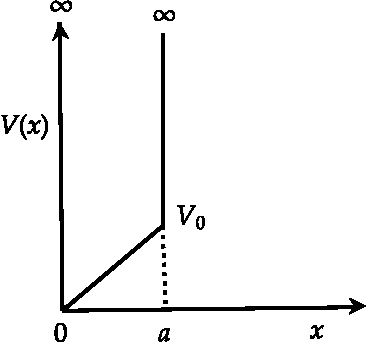
\includegraphics[height=3.3cm,width=4cm]{pert-crop}
		\caption{sliced infinite potential well}
		\label{}
	\end{figure}
	\begin{align*}
	\text{The first order }&\text{correction to the energy for the $\mathrm{n}=1$ state is}\\
	E_{1}^{(1)}&=\left\langle\psi_{1}^{0}\left|\frac{V_{0} x}{a}\right| \psi_{1}^{0}\right\rangle=\frac{V_{0}}{a} \frac{2}{a} \int_{0}^{a} x \sin ^{2} \frac{\pi x}{a} d x\\
	&=\frac{2 V_{0}}{a^{2}} \int_{0}^{a} \frac{x}{2}\left(1-\cos \frac{2 \pi x}{a}\right) d x=\frac{2 V_{0}}{a^{2}} \int_{0}^{a} \frac{x}{2} d x-\frac{2 V_{0}}{a^{2}} \int_{0}^{a} \frac{x}{2} \cos \frac{2 \pi x}{a} d x \\
	&=\frac{V_{0}}{2}+0=\frac{V_{0}}{2}\\
\text{	The first order correction }&\text{to the enegry for the $n=2$ state is}\\
	E_{2}^{(1)}&=\left\langle\psi_{2}^{0}\left|\frac{V_{0} x}{a}\right| \psi_{2}^{0}\right\rangle=\frac{V_{0}}{a} \frac{2}{a} \int x \sin ^{2} \frac{2 \pi x}{a} d x=\frac{V_{0}}{2}\\
	\text{The ground state and }&\text{first excited energies corrected upto first order are}\\
	\frac{\pi^{2} \hbar^{2}}{2 m a^{2}}&+\frac{V_{0}}{2} \text { and } \frac{2 \pi^{2} \hbar^{2}}{m a^{2}}+\frac{V_{0}}{2}
	\end{align*}
\end{answer}
\begin{exercise}
. A particle of mass ' $m$ ' moves in an infinite one-dimensional box of bottom ' $a$ ' with a potential dip as defined by
	$$
	\begin{aligned}
	&V(x)=\infty \text { for } x<0 \text { and } x>a \\
	&V(x)=-V_{0} \text { for } 0<x<\frac{a}{3} \\
	&V(x)=0 \text { for } \frac{a}{3}<x<a
	\end{aligned}
	$$
	Find the first order energy of the ground state.
\end{exercise}
\begin{answer}
For a particle in the infinite potential well defined by $V(x)=0$ for $0<x<a$ and $V(x)=\infty$ otherwise, the energy eigenvalues and normalized eigenfunctions are
$$
E_{n}=\frac{n^{2} \pi^{2} \hbar^{2}}{2 m a^{2}}, \psi_{n}=\sqrt{\frac{2}{a}} \sin \frac{n \pi x}{a}, \quad n=1,2,3, \ldots . .
$$
The perturbing Hamiltonian is $H$ ' $=-V_{0}$ for $0<x<a / 3$.
The first order energy correction to the ground state is\\
\begin{minipage}{0.5\textwidth}
$$
\begin{aligned}
E_{0}^{(1)} &=-\frac{2}{a} V_{0} \int_{0}^{a / 3} \sin ^{2} \frac{\pi x}{a} d x \\
&=-\frac{2}{a} V_{0} \int_{0}^{a / 3} \frac{1}{2}\left(1-\cos \frac{2 \pi x}{a}\right) d x \\
&=-\frac{V_{0}}{a}[x]_{0}^{a / 3}+\frac{V_{0}}{a} \frac{a}{2 \pi}\left[\sin \frac{2 \pi x}{a}\right]_{0}^{a / 3} \\
&=-\frac{V_{0}}{3}+\frac{V_{0}}{4 \pi} \times 0.866=-0.264 V_{0}
\end{aligned}
$$
The energy of the ground state corrected to first order is
$$
E_{1}^{\prime}=\frac{\pi^{2} \hbar^{2}}{2 m a^{2}}-0.264 V_{0}
$$	
\end{minipage}
\begin{minipage}{0.5\textwidth}
\begin{figure}[H]
	\centering
	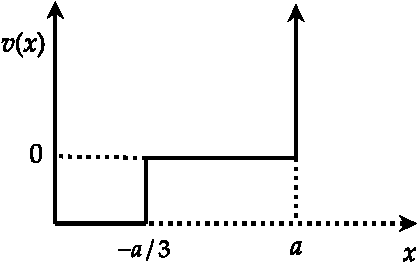
\includegraphics[height=3cm,width=4.5cm]{pert2}
	\caption{}
	\label{}
\end{figure}
\end{minipage}
\end{answer}
\section{The Variational Method}

There exist systems whose Hamiltonians are known, but they cannot be solved exactly or by a perturbative treatment. That is, there is no closely related Hamiltonian that can be solved exactly or approximately by perturbation theory because the first order is not sufficiently accurate. One of the approximation methods that is suitable for solving such problems is the variational method, which is also called the Rayleigh-Ritz method.  The variational method is useful for determining upper bound values for the eigenenergies of a system whose Hamiltonian is known whereas its eigenvalues and eigenstates are not known. It is particularly useful for determining the ground state. It becomes quite difficult to determine the energy levels of the excited states.\\\\
In the context of the variational method, one does not attempt to solve the eigenvalue problem
$$
\hat{H}|\psi\rangle=E|\psi\rangle,
$$
but rather one uses a variational scheme to find the approximate eigenenergies and eigenfunctions from the variational equation
$$
\delta E(\psi)=0
$$
where $E(\psi)$ is the expectation value of the energy in the state $|\psi\rangle$ :
$$
E(\psi)=\frac{\langle\psi|\hat{H}| \psi\rangle}{\langle\psi \mid \psi\rangle}
$$
$\text { If }|\psi\rangle \text { depends on a parameter } \alpha, E(\psi) \text { will also depend on } \alpha$\\
The variational method is particularly useful for determining the ground state energy and its eigenstate without explicitly solving the Schrödinger equation. Note that for any (arbitrary) trial function $|\psi\rangle$ we choose, the energy $E$ is always larger than the exact energy $E_{0}$ :
$$
E=\frac{\langle\psi|H| \psi\rangle}{\langle\psi \mid \psi\rangle} \geq E_{0}
$$
$\text { To calculate the ground state energy, we need to carry out the following four steps: }$
\begin{itemize}
	\item First, based on physical intuition, make an educated guess of a trial function that takes into account all the physical properties of the ground state (symmetries, number of nodes, smoothness, behavior at infinity, etc.). For the properties you are not sure about, include in the trial function adjustable parameters $\alpha_{1}, \alpha_{2}, \ldots$ (i.e., $\left.\left|\psi_{0}\right\rangle=\left|\psi_{0}\left(\alpha_{1}, a_{2}, \ldots\right)\right\rangle\right)$ which will account for the various possibilities of these unknown properties.
	\item Second, using $E(\psi)=\frac{\langle\psi|\hat{H}| \psi\rangle}{\langle\psi \mid \psi\rangle}$, calculate the energy; this yields an expression which depends on the parameters $\alpha_{1}, \alpha_{2}, \ldots$ :
	$$
	E_{0}\left(\alpha_{1}, \alpha_{2}, \ldots\right)=\frac{\left\langle\psi_{0}\left(\alpha_{1}, \alpha_{2}, \ldots\right)|\hat{H}| \psi_{0}\left(\alpha_{1}, \alpha_{2}, \ldots\right)\right\rangle}{\left\langle\psi_{0}\left(\alpha_{1}, \alpha_{2}, \ldots\right) \mid \psi_{0}\left(\alpha_{1}, \alpha_{2}, \ldots\right)\right\rangle} .
	$$
	In most cases $\left|\psi_{0}\left(\alpha_{1}, \alpha_{2}, \ldots\right)\right\rangle$ will be assumed to be normalized; hence the denominator of this expression is equal to 1 .
	\item Third, using the above equation search for the minimum of $E_{0}\left(\alpha_{1}, \alpha_{2}, \ldots\right)$ by varying the adjustable parameters $\alpha_{i}$ until $E_{0}$ is minimized. That is, minimize $E\left(\alpha_{1}, \alpha_{2}, \ldots\right)$ with respect to $\alpha_{1}, \alpha_{2}, \ldots$ :
	$$
	\frac{\partial E_{0}\left(\alpha_{1}, \alpha_{2}, \ldots\right)}{\partial \alpha_{i}}=\frac{\partial}{\partial \alpha_{i}} \frac{\left\langle\psi_{0}\left(\alpha_{1}, \alpha_{2}, \ldots\right)|\hat{H}| \psi_{0}\left(\alpha_{1}, \alpha_{2}, \ldots\right)\right\rangle}{\left\langle\psi_{0}\left(\alpha_{1}, \alpha_{2}, \ldots\right) \mid \psi_{0}\left(\alpha_{1}, \alpha_{2}, \ldots\right)\right\rangle}=0
	$$
	with $i=1,2, \ldots$. This gives the values of $\left(\alpha_{1_{0}}, \alpha_{2_{0}}, \ldots\right)$ that minimize $E_{0}$.
	\item - Fourth, substitute these values of $\left(\alpha_{1}, \alpha_{2_{0}}, \ldots\right)$ into $E_{0}\left(\alpha_{1_{0}}, \alpha_{2_{0}}, \ldots\right)$ to obtain the approximate value of the energy. The value $E_{0}\left(\alpha_{1_{0}}, \alpha_{2_{0}}, \ldots\right)$ thus obtained provides an upper bound for the exact ground state energy $E_{0}$. The exact ground state eigenstate $\left|\phi_{0}\right\rangle$ will then be approximated by the state $\left|\psi_{0}\left(\alpha_{1}, \alpha_{2_{0}}, \ldots\right)\right\rangle$.
\end{itemize}

 The variational method can also be used to find the approximate values for the energies of the first few excited states. For instance, to find the energy and eigenstate of the first excited state that will approximate $E_{1}$ and $\left|\phi_{1}\right\rangle$, we need to choose a trial function $\left|\psi_{1}\right\rangle$ that must be orthogonal to $\left|\psi_{0}\right\rangle$ :
$$\left\langle\psi_{1} \mid \phi_{0}\right\rangle=0$$

Then proceed as we did in the case of the ground state. That is, solve the variational equation $\delta E(\psi)=0$ for $\left|\psi_{1}\right\rangle:$
$$
\frac{\partial}{\partial \alpha_{i}} \frac{\left\langle\psi_{1}\left(\alpha_{1}, \alpha_{2}, \ldots\right)|\hat{H}| \psi_{1}\left(\alpha_{1}, \alpha_{2}, \ldots\right)\right\rangle}{\left\langle\psi_{1}\left(\alpha_{1}, \alpha_{2}, \ldots\right) \mid \psi_{1}\left(\alpha_{1}, \alpha_{2}, \ldots\right)\right\rangle}=0 \quad(i=1,2, \ldots) .
$$
Similarly, to evaluate the second excited state, we solve $\delta E(\psi)=0$ for  $\left|\psi_{2}\right\rangle$ and take into account the following two conditions:
$$
\left\langle\psi_{2} \mid \psi_{0}\right\rangle=0, \quad\left\langle\psi_{2} \mid \psi_{1}\right\rangle=0 .
$$
\begin{exercise}
 For the harmonic oscillator $V(x)=\frac{1}{2} m \omega^{2} x^{2}$, then choose a trial wave function $\psi(x, \alpha)=A e^{-\alpha x^{2}}$. Find the energy of ground state with the method of variational principle.
\end{exercise}
\begin{answer}
	\begin{align*}
		\text{From normalization condition }&\int_{-\infty}^{+\infty} \psi^{2} \psi d x=1,\text{ the value of }A=\left(\frac{2 \alpha}{\pi}\right)^{\frac{1}{4}}\\
	\text{The expectation value of kinetic energy for  }&\text{given wavefunction is}\langle T\rangle=\frac{\hbar^{2} \alpha}{2 m}\\
	\text{The expectation value of potential energy}\\
	\langle V\rangle&=\left(\frac{2 \alpha}{\pi}\right)^{2} \int_{-1}^{+1} \frac{1}{2} m \omega^{2} x^{2} e^{-2 \alpha x^{2}} d x\\
	&=\left(\frac{2 \alpha}{\pi}\right)^{\frac{1}{2}} \times \frac{1}{2} m \omega^{2} \int_{\infty}^{\infty} x^{2} e^{-2 \alpha x^{2}} d x
	=\frac{m \omega^{2}}{8 \alpha}\\
\text{	Then the expectation value of total energy is }\langle E\rangle&=\frac{\hbar^{2} \alpha}{2 m}+\frac{m \omega^{2}}{8 \alpha}\\
	\frac{d E}{d \alpha}&=0, \frac{\hbar^{2}}{2 m}-\frac{m \omega^{2}}{8 \alpha^{2}}=0, \alpha_{0}=\frac{m \omega}{2 \hbar}\\
	\text{putting the value of }&\alpha_{0} \quad \alpha_{0}=\frac{m \omega}{2 \hbar} \Rightarrow\langle E\rangle=\frac{\hbar \omega}{2}
	\end{align*}
\end{answer}
\begin{exercise}
 Find the energy eigen value for the ground state if particle is confined into $1-D$ infinite potential box of width ' $a$ ' centered at $\frac{a}{2}$ by taking trial wavefunction. $\psi=A x(a-x)$.
\end{exercise}
\begin{answer}$\left. \right. $\\
	\begin{minipage}{0.5\textwidth}
		\begin{align*}	
		\text{For normal}&\text{ization }|A|^{2} \int_{0}^{a} x^{2}(a-x)^{2} d x=1 \Rightarrow A=\left(\frac{30}{a^{5}}\right)^{\frac{1}{2}}\\
		\text{The expectation }&\text{value of kinetic energy}\\
		\langle T\rangle&=\int_{0}^{a}\left(\frac{30}{a^{5}}\right)^{\frac{1}{2}} x(a-x) \frac{-\hbar}{2 m} \frac{\partial^{2}}{\partial x^{2}}\left(\frac{30}{a^{5}}\right)^{\frac{1}{2}} x(a-x) d x \\
		&=\frac{\hbar^{2}}{m}\left(\frac{30}{a^{5}}\right) \frac{a^{3}}{6}=\frac{5 \hbar^{2}}{m a^{2}}\\
	\text{	The expectation }&\text {value of potential energy is $\langle V\rangle=0$}\\
		\langle E\rangle&=\langle T\rangle+\langle V\rangle=\frac{5 \hbar^{2}}{m a^{2}}\\
	\text{	(constant value)}
		\end{align*}
	\end{minipage}
 \begin{minipage}{0.4\textwidth}
 \begin{figure}[H]
 	\centering
 	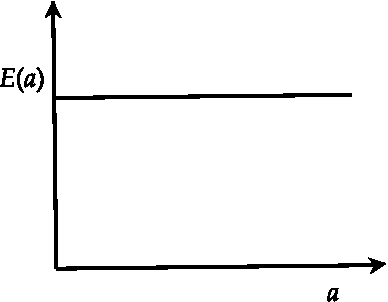
\includegraphics[height=3cm,width=4cm]{var-crop}
 \end{figure}	
 \end{minipage}
\end{answer}
\section{The WKB Appoximation Method}
The Wentzel-Kramers-Brillouin (WKB) method is useful for approximate treatments of systems with slowly varying potentials; that is, potentials which remain almost constant over a region of the order of the de Broglie wavelength. In the case of classical systems, this property is always satisfied since the wavelength of a classical system approaches zero. The WKB method can thus be viewed as a semiclassical approximation.\\
\textbf{General Formalism}\\
Consider the motion of a particle in a time-independent potential $V(\vec{r}) ;$ the Schrödinger equation for the corresponding stationary state is
	$$
	\begin{aligned}
	-\frac{\hbar^{2}}{2 m} \nabla^{2} \psi(\vec{r})+V(\vec{r}) \psi(\vec{r})&=E \psi(\vec{r})\\
\text{	or}\qquad
	\nabla^{2} \psi(\vec{r})+\frac{1}{\hbar^{2}} p^{2}(\vec{r}) \psi(\vec{r})&=0
\end{aligned}
$$
where $p(\vec{r})$ is the classical momentum at $\vec{r}: p(\vec{r})=\sqrt{2 m(E-V(\vec{r}))}$. If the particle is moving in a region where $V(\vec{r})$ is constant, the solution of schrodinger equation is of the form $\psi(\vec{r})=A e^{\pm i \vec{p} \cdot \vec{r} / \hbar} .$ But how does one deal with those cases where $V(\vec{r})$ is not constant? The WKB method provides an approximate treatment for systems whose potentials, while not constant, are slowly varying functions of $\vec{r}$. That is, $V(\vec{r})$ is almost constant in a region which extends over several de Broglie wavelengths; we may recall that the de Broglie wavelength of a particle of mass $m$ and energy $E$ that is moving in a potential $V(\vec{r})$ is given by $\lambda=h / p=h / \sqrt{2 m(E-V(\vec{r}))}$.\\
In essence, the WKB method consists of trying a solution to schrodinger rquation
$$
\psi(\vec{r})=A(\vec{r}) e^{i S(\vec{r}) / \hbar},
$$
Where $A(\vec{r})$ is the amplitude and $S(\vec{r})$ is the phase both are real functions and yet to be determined\\
Substituting the value of $
\psi(\vec{r})=A(\vec{r}) e^{i S(\vec{r}) / \hbar},
$ in to schrodinger equation we will get\\
$$A\left[\frac{\hbar^{2}}{A} \nabla^{2} A-(\vec{\nabla} S)^{2}+p^{2}(\vec{r})\right]+i \hbar\left[2(\vec{\nabla} A) \cdot(\vec{\nabla} S)+A \nabla^{2} S\right]=0$$
The real and imaginary parts of this equation must vanish separately:
$$
\begin{gathered}
(\vec{\nabla} S)^{2}=p^{2}(\vec{r})=2 m(E-V(\vec{r})) \\
2(\vec{\nabla} A) \cdot(\vec{\nabla} S)+A \nabla^{2} S=0
\end{gathered}
$$
To illustrate the various aspects of the WKB method, let us consider the simple case of the one-dimensional motion of a single particle. We can thus reduce the above two equations, respectively, to
	$$
	\begin{aligned}
		\frac{d S}{d x}&=\pm \sqrt{2 m(E-V)}=\pm p(x) \\
		2\left(\frac{d}{d x} \ln A\right) p(x)&+\frac{d}{d x} p(x)=0\\
	\text{From these two equations }&\text{$A(\vec{r})$ ,$S(\vec{r})$ can be found.}\\
	S(x)&=\pm \int d x \sqrt{2 m(E-V(x))}=\pm \int p(x) d x\\
	\frac{d}{d x}[2 \ln A+\ln p(x)]=0\\
\text{	which in turn leads to}\qquad
	A(x)&=\frac{C}{\sqrt{|p(x)|}}\\
\text{	we will get the solution by }&\text{substituting the values of $A(\vec{r})$ ,$S(\vec{r})$ in to }	\psi(\vec{r})\\
	\psi_{\pm}(x)&=\frac{C_{\pm}}{\sqrt{|p(x)|}} \exp \left[\pm \frac{i}{\hbar} \int^{x} p\left(x^{\prime}\right) d x^{\prime}\right] 
\end{aligned}
$$
The amplitude of this wave function is proportional to $1 / \sqrt{p(x)}$; hence the probability of finding the particle between $x$ and $x+d x$ is proportional to $1 / p(x)$. This is what we expect for a "classical" particle because the time it will take to travel a distance $d x$ is proportional to the inverse of its speed (or its momentum).
\par We can now examine two separate cases corresponding to $E>V(x)$ and $E<V(x)$. First, let us consider the case $E>V(x)$, which is called the classically allowed region. Here $p(x)$ is a real function; the most general solution  is a combination of $\psi_{+}(x)$ and $\psi_{-}(x)$ :
$$
\psi(x)=\frac{C_{+}}{\sqrt{p(x)}} \exp \left[\frac{i}{\hbar} \int^{x} p\left(x^{\prime}\right) d x^{\prime}\right]+\frac{C_{-}}{\sqrt{p(x)}} \exp \left[-\frac{i}{\hbar} \int^{x} p\left(x^{\prime}\right) d x^{\prime}\right]
$$
Second, in the case where $E<V(x)$, which is known as the classically forbidden region, the momentum $p(x)$ is imaginary and the exponents of become real:
$$
\psi(x)=\frac{C_{-}^{\prime}}{\sqrt{|p(x)|}} \exp \left[-\frac{1}{\hbar} \int_{x}\left|p\left(x^{\prime}\right)\right| d x^{\prime}\right]+\frac{C_{+}^{\prime}}{\sqrt{|p(x)|}} \exp \left[\frac{1}{\hbar} \int^{x}\left|p\left(x^{\prime}\right)\right| d x^{\prime}\right]
$$
But what about the structure of the wave function near the regions $E \simeq$ $V(x)$ ? At the points $x_{i}$, we have $E=V\left(x_{i}\right)$; hence the momentum $(9.167)$ vanishes, $p\left(x_{1}\right)=0$. These points are called the classical turning points, because classically the particle stops at $x_{i}$ and then turns back to resume its motion in the opposite direction. At these points the wave function $\psi_{\pm}(x)$ becomes infinite since $p\left(x_{i}\right)=0$. 
\subsection{ W.K.B. Approximation Rules for Bound State Energy :}
\begin{enumerate}
	\item  If both walls are smooth $\Rightarrow \oint p_{x} d x=\left(n+\frac{1}{2}\right) h \quad n=0,1,2 \ldots$
	$$
	2 \int_{x_{1}}^{x_{2}} p_{x} d x=\left(n+\frac{1}{2}\right) h \text { where } x_{1} \text { and } x_{2} \text { are turning point. }
	$$
	\item If one wall is smooth \& one wall is rigid 
	$$
	\begin{aligned}
			\int_{x_{1}}^{x_{2}} p_{x} d x&=\left(n+\frac{\dot{3}}{4}\right) \pi \hbar \quad\\
		\text{where }x_{1}&\text{ and }x_{2}\text{ are turning point}\\
		n&=0,1,2,3 \ldots . \\
		&=\left(n+1+\frac{3}{4}-1\right) \pi \hbar=\left(n-\frac{1}{4}\right) \pi \hbar, \quad n=1,2,3 \ldots .
	\end{aligned}
	$$
	  \item When both walls are rigid:
	  $\int_{x_{1}}^{x_{2}} p_{x} d x=(n+1) \pi \hbar \quad$ \\
	  where $x_{1}$ and $x_{2}$ are turning point $n=0,1,2, \ldots . .$
	  $$
	  \text { if }(n+1)=m \quad m=1,2,3 \ldots
	  $$
\end{enumerate}


\section{Time Dependent Perturbation Theory}
To study the structure of molecular and atomic systems, we need to know how electromagnetic radiation interacts with these systems. Molecular and atomic spectroscopy deals in essence with the absorption and emission of electromagnetic radiation by molecules and atoms. As a system absorbs or emits radiation, it undergoes transitions from one state to another.\\
Time-dependent perturbation theory is most useful for studying processes of absorption and emission of radiation by atoms or, more generally, for treating the transitions of quantum systems from one energy level to another.\\\\
\par Time evolution problem uses pertubration method to find the solution. If the hamiltonian is time dependent we can write, the totl H
$$H=H_0+H^\prime$$
Where $H_0$ is time independent unperturbed term. It constitutes major part of $H$.
Its eigen values and ortho normalized eigen function are known.
$$\therefore H_0u_n=E_n u_n\quad \int u_m u_n d\tau=\delta_{mn}$$
Since it is a time evolution problem we use time dependent schoodinger equation \\
So,
	$$
	\begin{aligned}
	H\psi&=E\psi\\
	H&=H_0+H^\prime\quad E=-i\hbar\frac{ d}{dt}\\
	\therefore\quad \frac{i\hbar d \psi}{dt}&=H_0\psi+H^\prime\psi
\end{aligned}
$$





Which has the solution of the form.
$$\psi(x,t)=\sum_{n}a_n(t)u_n(x)e^{\frac{-i}{\hbar }E_nt}$$
Where $|a_n(t)|^2$ is the probability with which the system described by $\psi(x,t)$ in an energy eigen state $u_n(x)$\\\\
on substituting the the value of $\psi(x,t)$ in schrodinger equation 
$$\implies\sum_{n}(i\hbar \dot{a}_n(t)+E_na_n)u_n e^{\frac{-i}{\hbar} E_nt}=\sum_{n}(H_0u_n+H^\prime u_n)a_ne^{\frac{-i}{\hbar}E_nt}$$
Since $H_0u_n=E_nu_n$ the term get cancelled on both side\\
$$\sum_{n}i\hbar\dot{a}_nu_ne^{\frac{-i}{\hbar}E_nt}=\sum_{n}H^\prime u_n a_n e^{\frac{-i}{\hbar}E_nt}$$
Multiplying with $u_f^*$ and integrating\\
$$ \int i\hbar \sum_{n} \dot{a}_n u_n u_f^* e^{\frac{-i}{\hbar}E_nt}d\tau=\sum_{n}\int u_f^*H^\prime u_na_ne^{\frac{-i}{\hbar}E_nt}d\tau$$
$$ i\hbar{\dot{a}}_f e^{\frac{-i}{\hbar}E_ft}=\sum_{n}a_n {H\prime} _{fn} e^{\frac{-i}{\hbar}E_nt}\hspace{2cm}
\int u_f^* u_n d\tau=\delta_{fn}$$
$$ \dot{a}_f =(i\hbar)^{-1}\sum a_n H^\prime_{fn}e^{\frac{-i}{\hbar}[E_f-E_n]t}\hspace{2cm}\int u_f^* H^\prime u_n d\tau=H^\prime_{fn}$$
$$\therefore \dot{a}_f=(i\hbar)^{-1}\sum_n a_n H^\prime_{fn}e^{i\omega_{fn}t}\hspace{2cm}E_f-E_n=\omega_{fn}\hbar
$$
Since $H^\prime$ are small $a_f$ can be expanded as \\
$$a_f(t)=a_f^0+a_f^1+a_f^2+....$$
On substituting this in $\dot{a}_f$ and equating terms of the same order on both sides,we get
$$\dot{a}_f^{(0)}=0\quad \dot{a}_f^{(r+1)}(t)=(l\hbar)^{-1}\sum_n
a_n^{(r)}H_{fn}^\prime e^{i\omega_{fn}t}$$
By substituting the initial condition $r=0$ we get
$$\dot{a}_f^{(1)}=(i\hbar)^{-1}H^{\prime}_{fi}e^{i\omega_{fn}t}$$
$$\therefore a_f^{(1)}(t)=(ih)^{-1}\int_{0}^{t}H^\prime_{fl}(t^\prime)e^{i\omega_{fi}t^{\prime}}dt^\prime$$
In many cases\\
$$H^\prime _{fi}(t)=H_{fi}^{\prime 0}f(t)$$
Where $H^{\prime 0}$ is time independent\\
$$\therefore a_f^{(1)}(t)=(i\hbar)^{-1}H^{10}_{fi}\int_{0}^{t}f(t^\prime)e^{i\omega_{fi}t^{\prime}}dt^\prime$$
\subsection{First Order Transition: Constant Perturbation }
Probability of transition from $i $ to all states $f\neq i$ is much less than unit
$$ \sum^\prime|a^\prime_f(t)|^2<<1$$
\textbf{(a)\quad Transition Probability }\\
We now consider the specific case of a perturbation $H^\prime$ which lasts from time $0  $ to $t$ and is constant during this period.\\
$$\therefore \quad  a_f(t)=(ih)^{-1}\int H^\prime _{fi}e^{i\omega_{fi}t}dt $$ 
$\therefore \quad H^\prime_{fi}$ is constant\\
$$a_f(t)=(i\hbar)^{-1}H^\prime_{fi}\int e^{i\omega_{fi}t}dt$$
$$=(i\hbar)^{-1}H^\prime_{fi}\frac{e^{i\omega_{fi}t}-1}{i\omega_{fi}}=-H^\prime_{fi}\frac{e^{i\omega_{fi}t}-1}{\hbar\omega_{fi}}$$
$$|a_f(t)|^2=\frac{|H_{fi}|^2}{\hbar^2}\frac{4\sin^2\frac{1}{2}\omega_{fi}t}{\omega_{fi}^2}$$

Trnsition probability from $i$ to $f$ deosnot change monotonically with time but varies simple harmonically from zero to maximum ($=\frac{4|H^\prime_{fi}|^2}{\hbar^2\omega_{fi}^2}$) with frequency equal to Bohr frequency $\frac{\omega_{fi}}{2\pi}$. When smaller the energy difference $E_f-E_i=\hbar\omega_{fi}$ Between the pairs larger the maximum value of probability.\\
The behaviour of the factor $\frac{4}{(\omega_{fi})^2}\sin^2\frac{1}{2}\omega_{fi}t$ is drawn.\\
\begin{figure}[H]
	\centering
	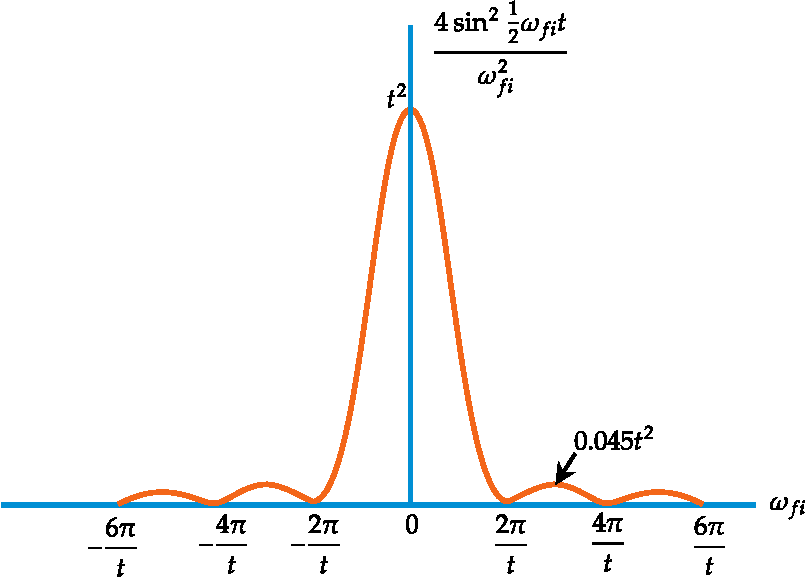
\includegraphics[height=5cm,width=8.5cm]{Q-1}
\end{figure}
The main peak of the curve occurs at $\omega_{fi}=0$ is of height $t^2$\\
$\therefore$ We see that the transition from $i$ take place with appreciable probability only to those level $f$ such that $\omega_{fi}$ falls under the main peak: $|\omega_{fi}|\leq \frac{2\pi}{t}$.In other words the magnitude of the energy difference
$|\hbar\omega_{fi}|$ between the initial and final states is very unlikely to be significally higher than $\hbar(\frac{2\pi}{t})=\frac{h}{t}$.This result is  generally considered as an expression of an energy time uncertainity relation .
	$$
	\begin{aligned}
	\hbar\omega_{fi}\leq\frac{\hbar2\pi}{\tau}\quad\hbar&=\frac{\hbar}{2\pi}\\
	\Delta E\leq \frac{\hbar}{\Delta t}\quad \Delta E\Delta t&\approx h
\end{aligned}
$$



Energy time uncertainity relation\\
\textbf{(b)\quad Closely Packed Levels}\\
Suppose there are many $f$ levels within the energy level $\Delta E$ Covered by the main peak, then,\\
$$\sum_{f}|a_f(t)|^2=\frac{H_{fi}}{\hbar^2}\sum_{f}\frac{4\sin^2 \frac{1}{2}\omega_{fi}t}{\omega^2_{fi}}$$
Summation is over $f$\\
If spacing are very close summation can be changed in to integration such as,
$$\sum_{f}.....\implies \int(E_f)dE_f\rightarrow\rho(E_f)\int dE_f$$
Where $\rho(E_f)$ is the density of states that is the number of state around the energy. 
Number of state with energy with in $d(E_f)=d_{nf}=\rho(E_f)dE_f \rho(f)$ is constant.
	$$
	\begin{aligned}
	\therefore \sum_{f}|a^{(1)}_f(t)|^2&=\frac{|H_{fi}|^2}{\hbar^2}\rho(E_f)\int\frac{4\sin^2\frac{1}{2}\omega_{fi}t}{(\omega_{fi})^2}dE_f\\
	\hbar\omega_{fi}&=E_f-E_i\\
	\hbar d\omega_{fi}&=dE_f\\
	 d\omega_{fi}&=\frac{dE_f}{\hbar}\\
	\therefore\sum_{f}|a^{1}_f(t)|^2&=\frac{|H_{fi}|^2}{\hbar^2}\rho(E_f)\int\frac{4\sin^2\frac{1}{2}\omega_{fi}t}{(\omega_{fi})^2}d\omega_{fi}\\
	\text{Since} \quad 2t\int_{-\infty}^{\infty}x^{-2}\sin^2xdx&=2\pi t\\
	\sum_{f}|a^{1}_f(t)|^2&=\frac{2\pi}{\hbar}t|H_{fi}|^2\rho(E_f)\\
	\therefore \text{Transition probability /unit time}\\
	\frac{1}{t}\sum_{f}a^{(1)}_f(t)|^2&=\frac{2\pi}{\hbar}t|H_{fi}|^2\rho(E_f)\\
	\text{This formula is called }&\textcolor{red}{\text{'Fermi Golden rule'}}
\end{aligned}
$$
\subsection{Harmonic Perturbation}
\textbf{(a)Amplitude for Transition With Change of Energy}\\
We shall now consider a harmonic perturbation .
consider a perturbation of the type
\begin{align*}
H^\prime&=H^{\prime o}e^{-i\omega t} (\omega>0) \quad \quad  H^\prime=H^{\prime o}f(t)
\end{align*}
supposed to act during the time interval (o,t),Then
\begin{align*}
a^{\prime}_f (t)&=(i\hbar)^{-1}H^{\prime o}_{fi}\int f(t)e^{i\omega_{fi} t}  dt \quad \quad  f(t)=e^{-i\omega t}\\
\intertext{The first order transition amplitude is}
a_f(t)& =-H^{\prime o}_{fi}\ \frac{e^{l(\omega_{fi}-\omega)t}-1}{(\omega_{fi}-\omega)\hbar}
\end{align*}
For large $t$ only those transitions with $\omega_{fi}-\omega=0$ or $E_f-E_i=\hbar \omega$  are possible with appreciable probability.\\
This means that perturbation can induce transition from $E_i$ to the level $E_f$ whose energy is higher than $E_i$ by $\hbar \omega$
Such a transition may be described as absorption of energy $\hbar \omega$ by the system from the purturbing agency\\
For the hermitian congugate of $H^\prime$\\
$$ H^{1\dagger}=(H^{\prime o})^\dagger e^{i\omega t}$$
Which makes the charges in transition amplitude for the factor $(H^{\prime o}_{fi})^\dagger=(H^{\prime o}_{if})$ as the over all factor and it induce the transition.
$$\omega_{fi}+\omega=0\quad \text{or }E_f-E_i=-\hbar\omega $$
In this case $E_f$ is lower and that is energy $\hbar\omega$ is given away by the system to the purturbing agency. ie emission.\\
The actual perturbation can be written as 
$$ H^\prime=H^{\prime o}e^{-i \omega t}+(H^{\prime o})^\dagger e^{+\omega t}$$
\textbf{(b) Transition Induced by Incoherent Spectrum of Perturbing Frequencies}\\
As long as the perturbation contains only single frequency ,the transition probability oscillates with time as ($\omega_{fi}\mp\omega$) instead of $\omega_{fi}$.\\
However the transition probability preportional to time can arise under the following conditions\\
(i)The perturbation involves a whole spectrum of frequencies $\omega$ which are so closely spaced that very many such frequencies are contained with in the intervel (1/t).\\
(ii)These are incoherent in the sense that the phase of the different frequency componets are unrelated to each other.\\
(iii)The magnitude of these perturbations and the spacing of the frequencies are smooth function of $\omega$.\\\\
Consider the second situation of incoherent frequency.To determine the total transition probability induced by the whole spectrum of frequencies one simply add up the probabilities arising from the different frequency components.Condition (i) then enables this sum to be replaced by an integral.Thus the total transition probability will be 
$$
\begin{aligned}
\sum_{\omega} |a_f(t,\omega)|^2 &= \sum_{\omega}  \frac{|H^{\prime o}_{fi}(\omega)|^2}{\hbar^2}\ \frac{4 \sin^2\frac{1}{2}(\omega_{fi}+\omega)t}{(\omega_{fi}-\omega)^2}\\
&=\int \frac{|H^{\prime o}_{fi}(\omega)|^2}{\hbar^2}\frac{4 \sin^2\frac{1}{2}(\omega_{fi}+\omega)t}{(\omega_{fi}-\omega)^2}\rho (\omega)\ d\omega
\end{aligned}
$$
$|H_{fi}(\omega)|^2$ and $\rho(\omega)$ Varies smothly with $\omega$ and almost constant in the intervel $\frac{1}{t}$ around $\omega=\omega_{fi}$ both can be taken out integral and after integrating we get,\\
Transition probability per unit time
$$  = \frac{2\pi}{\hbar^2}|H^{\prime o}_{fi}(\omega_{fi})|^2 \rho (\omega_{fi})$$
here the total perturbration can be written as,
$$H^\prime = H^{\prime o}(\omega)e^{-i\omega t}+ H^{\prime o}(-\omega)e^{i\omega t}$$
with $H^{\prime o}(-\omega)=[H^{\prime o}(\omega)]^\dagger$ to ensure hermiticity.
In order to consider the both term the summation should be done for $+\omega$ and $-\omega$ with
$$ H^{\prime o}_{fi}(\omega)=H^{\prime o}_{if}(\omega),\rho(\omega)=\rho(-\omega)$$
$\therefore$ for upward transition $E_f>E_n$ from $i$ to $f$ and downward transition from $f$ to $i$ $E_f<E_n$
probability/unit time is 
$$ =\frac{2\pi}{\hbar^2}|H^{\prime_0}_{fi}(\omega_{fi})|^2 \rho(\omega_{fi})\text{ and } \frac{2\pi}{\hbar^2}|H^{\prime_0}_{fi}(-\omega_{fi})|^2\rho(-\omega_{fi})$$
Since $$\omega_{mn}=-\omega_{nm}$$
These two probability/unit time are equal.\\
$\therefore$ Probabilities for upward and downward transition between a given pair of levels induced by hermition pertubration are identical.







\section{Pictures of Quantum Mechanics}
Each class of representation also called a picture differs from others in the way it treats the time evolution of the system.Schrodinger picture is useful when describing phenomena with time independent Hamiltonians,whereas the interaction and heisenberg pictures are useful when describing phenomena with time dependent Hamiltonians.
\subsection{The Schrodinger Picture}
In describing quantum dynamics, we have been using so far the Schrödinger picture in which state vectors depend explicitly on time, but operators do not:
$$
i \hbar \frac{d}{d t}|\psi(t)\rangle=\hat{H}|\psi(t)\rangle,
$$
where $|\psi(t)\rangle$ denotes the state of the system in the Schrödinger picture.The  time evolution of a state $|\psi(t)\rangle$ can be expressed by means of the propagator, or time-evolution operator, $\hat{U}\left(t, t_{0}\right)$, as follows:
$$
|\psi(t)\rangle=\hat{U}\left(t, t_{0}\right)\left|\psi\left(t_{0}\right)\right\rangle,
$$
with
$$
\hat{U}\left(t, t_{0}\right)=e^{-i\left(t-t_{0}\right) \hat{H} / \hbar}
$$
The operator $\hat{U}\left(t, t_{0}\right)$ is unitary,
$$
\hat{U}^{\dagger}\left(t, t_{0}\right) \hat{U}\left(t, t_{0}\right)=I
$$
and satisfies these properties:
$$
\begin{gathered}
\hat{U}(t, t)=I \\
\hat{U}^{\dagger}\left(t, t_{0}\right)=\hat{U}^{-1}\left(t, t_{0}\right)=\hat{U}\left(t_{0}, t\right) \\
\hat{U}\left(t_{1}, t_{2}\right) \hat{U}\left(t_{2}, t_{3}\right)=\hat{U}\left(t_{1}, t_{3}\right)
\end{gathered}
$$
\subsection{The Heisenberg Picture}
In this picture the time dependence of the state vectors is completely frozen. The Heisenberg picture is obtained from the Schrödinger picture by applying $\hat{U}$ on $|\psi(t)\rangle_{H}$ :
$$
|\psi(t)\rangle_{H}=\hat{U}^{\dagger}(t)|\psi(t)\rangle=|\psi(0)\rangle,
$$
where $|\psi(t)\rangle$ and $\hat{U}^{\dagger}(t)$ can be obtained from scrodinger picture by setting $t_{0}=0$ : $\hat{U}^{\dagger}(t)=\hat{U}^{\dagger}\left(t, t_{0}=0\right)=e^{i t \hat{H} / \hbar}$ and $|\psi(t)\rangle=\hat{U}(t)|\psi(0)\rangle$, with $\hat{U}(t)=e^{-i t \hat{H} / \hbar}$. Thus, we can rewrite \\
$$\psi(t)\rangle_{H}=e^{i t \hat{H} / \hbar}|\psi(t)\rangle$$
As $|\psi\rangle_{H}$ is frozen in time we have: $d|\psi\rangle_{H} / d t=0$. Let us see how the expectation value of an operator $\hat{A}$ in the state $|\psi(t)\rangle$ evolves in time:
$$
\left.\langle\psi(t)|\hat{A}| \psi(t)\rangle=\left\langle\psi(0)\left|e^{i t \hat{H} / \hbar} \hat{A} e^{-i t \hat{H} / \hbar}\right| \psi(0)\right\rangle=\left\langle\psi(0)\left|\hat{A}_{H}(t)\right| \psi(0)\right\rangle=H\left\langle\psi\left|\hat{A}_{H}(t)\right| \psi\right\rangle\right\rangle_{H},
$$
where $\hat{A}_{H}(t)$ is given by\\
$$\hat{A}_{H}(t)=\hat{U}^{\dagger}(t) \hat{A} \hat{U}(t)=e^{i t \hat{H} / \hbar} \hat{A} e^{-i t \hat{H} / \hbar}$$
Schrödinger and the Heisenberg pictures coincide at $t=0,5$ \\
\textbf{Heisenberg Equation of Motion}\\
$$\frac{d\hat{A}_H}{dt}=\frac{1}{i\hbar}\left[\hat{A}_H,\hat{H}\right] $$ 
\subsection{The Interaction Picture}
The interaction picture, also called the Dirac picture, is useful to describe quantum phenomena with Hamiltonians that depend explicitly on time. In this picture both state vectors and operators evolve in time. We need, therefore, to find the equation of motion for the state vectors and for the operators.\\
\textbf{Equation of Motion of State Vectors}\\
State vectors in the interaction picture are defined in terms of the Schrödinger states | $\psi(t)\}$ by
$$
|\psi(t)\rangle_{I}=e^{i t \hat{H}_{0} / \hbar}|\psi(t)\rangle .
$$
If $t=0$ we have $|\psi(0)\rangle_{I}=|\psi(0)\rangle$. The time evolution of $|\psi(t)\rangle$ is governed by the Schrödinger equation $(10.1)$ with $\hat{H}=\hat{H}_{0}+\hat{V}$ where $\hat{H}_{0}$ is time independent, but $\hat{V}$ may depend on time.
To find the time evolution of $|\psi(t)\rangle_{I}$, we need the time derivative 
$$
\begin{aligned}
i \hbar \frac{d|\psi(t)\rangle_{I}}{d t} &=-\hat{H}_{0} e^{i t \hat{H}_{0} / \hbar}|\psi(t)\rangle+e^{i t \hat{H}_{0} / \hbar}\left(i \hbar \frac{d|\psi(t)\rangle}{d t}\right) \\
&=-\hat{H}_{0}|\psi(t)\rangle_{I}+e^{i t \hat{H}_{0} / \hbar} \hat{H}|\psi(t)\rangle
\end{aligned}
$$
$\text { Since } \hat{H}=\hat{H}_{0}+\hat{V} \text { and }$
$$\begin{gathered}
e^{i H_{0} t / \hbar} \hat{V}=\left(e^{i t \hat{H}_{0} / \hbar} \hat{V} e^{-i t \hat{H}_{0} / \hbar}\right) e^{i t \hat{H}_{0} / \hbar}=\hat{V}_{I}(t) e^{i t \hat{H}_{0} / \hbar}, \\
\hat{V}_{I}(t)=e^{i t \hat{H}_{0} / \hbar} \hat{V} e^{-i t \hat{H}_{0} / \hbar},
\end{gathered}$$
we can rewrite\\
$$\begin{gathered}
i \hbar \frac{d|\psi(t)\rangle_{I}}{d t}=-\hat{H}_{0}|\psi(t)\rangle_{I}+\hat{H}_{0} e^{i t \hat{H}_{0} / \hbar}|\psi(t)\rangle+\hat{V}_{I}(t) e^{i t \hat{H}_{0} / \hbar}|\psi(t)\rangle, \\
i \hbar \frac{d|\psi(t)\rangle_{I}}{d t}=\hat{V}_{I}(t)|\psi(t)\rangle_{I} .
\end{gathered}$$
This is the Schrödinger equation in the interaction picture. It shows that the time evolution of the state vector is governed by the interaction $\hat{V}_{I}(t)$.\\
\textbf{Equation of Motion for the Operators}\\
The interaction representation of an operator $\hat{A}_{J}(t)$ is given, in terms of its Schrödinger representation by
$$
\hat{A}_{I}(t)=e^{i \hat{H}_{0} t / \hbar} \hat{A} e^{-i \hat{H}_{0} t / \hbar}
$$
Calculating the time derivative of $\hat{A}_{I}(t)$ and since $\partial \hat{A} / \partial t=0$, we can show the time evolution of $\hat{A}_{I}(t)$ is governed by $\hat{H}_{0}$ :
$$
\frac{d \hat{A}_{I}(t)}{d t}=\frac{1}{i \hbar}\left[\hat{A}_{I}(t), \hat{H}_{0}\right]
$$
This equation is similar to the Heisenberg equation of motion except that $\hat{H}$ is replaced by $\hat{H}_{0}$. The basic difference between the Heisenberg and interaction pictures:In the Heisenberg picture it is $\hat{H}$ that appears in the exponents,whereas in the interaction picture it is $\hat{H}_0$ that appears.\\
\textbf{Conclusion}\\
 we have seen that with in the schrodinger picture ,the states depends on time but not operators;In the Heisenberg picture only operators depends explicitly on time,state vectors are frozen in time.The interaction picture however is intermediate between the Schrodinger and the Heisenberg pictures ,since both state vectors and operators evolve with time.\\
 \newpage
 \begin{abox}
 	Practice set 1
 	\end{abox}
 \begin{enumerate}
 \begin{minipage}{\textwidth}
 	\item If the perturbation $H^{\prime}=a x$, where $a$ is a constant, is added to the infinite square well potential
 	$$
 	V(x)=\left\{\begin{array}{lll}
 	0 & \text { for } & 0 \leq x \leq \pi \\
 	\infty & & \text { otherwise }
 	\end{array}\right.
 	$$
 	The correction to the ground state energy, to first order in $a$, is
 	\exyear{NET JUNE 2011}
 \end{minipage}
 \begin{tasks}(4)
 	\task[\textbf{A.}] $\frac{a \pi}{2}$
 	\task[\textbf{B.}]$a \pi$
 	\task[\textbf{C.}]$\frac{a \pi}{4}$
 	\task[\textbf{D.}]$\frac{a \pi}{\sqrt{2}}$
 \end{tasks}
\begin{minipage}{\textwidth}
	\item A particle in one dimension moves under the influence of a potential $V(x)=a x^{6}$, where $a$ is a real constant. For large $n$ the quantized energy level $E_{n}$ depends on $n$ as:
	\exyear{NET JUNE 2011}
\end{minipage}
\begin{tasks}(2)
	\task[\textbf{A.}] $E_{n} \sim n^{3}$
	\task[\textbf{B.}]$E_{n} \sim n^{4 / 3}$
	\task[\textbf{C.}]$E_{n} \sim n^{6 / 5}$
	\task[\textbf{D.}]$E_{n} \sim n^{3 / 2}$
\end{tasks}
\begin{minipage}{\textwidth}
	\item The perturbation $H^{\prime}=b x^{4}$, where $b$ is a constant, is added to the one dimensional harmonic oscillator potential $V(x)=\frac{1}{2} m \omega^{2} x^{2}$. Which of the following denotes the correction to the ground state energy to first order in $b$ ?
	Hint: The normalized ground state wave function of the one dimensional harmonic oscillator potential is $\psi_{0}=\left(\frac{m \omega}{\hbar \pi}\right)^{1 / 4} e^{-m \omega x^{2} / 2 \hbar} .$ You may use the following integral $\left.\int_{-\infty}^{\infty} x^{2 n} e^{-a x^{2}} d x=a^{-n-\frac{1}{2}} \Gamma\left(n+\frac{1}{2}\right)\right]$
	\exyear{NET DEC 2011}
\end{minipage}
\begin{tasks}(2)
	\task[\textbf{A.}] $\frac{3 b \hbar^{2}}{4 m^{2} \omega^{2}}$
	\task[\textbf{B.}]$\frac{3 b \hbar^{2}}{2 m^{2} \omega^{2}}$
	\task[\textbf{C.}]$\frac{3 b \hbar^{2}}{2 \pi m^{2} \omega^{2}}$
	\task[\textbf{D.}]$\frac{15 b \hbar^{2}}{4 m^{2} \omega^{2}}$
\end{tasks}
\begin{minipage}{\textwidth}
	\item A constant perturbation as shown in the figure below acts on a particle of mass $m$ confined in an infinite potential well between 0 and $L$.\\
	\begin{figure}[H]
		\centering
		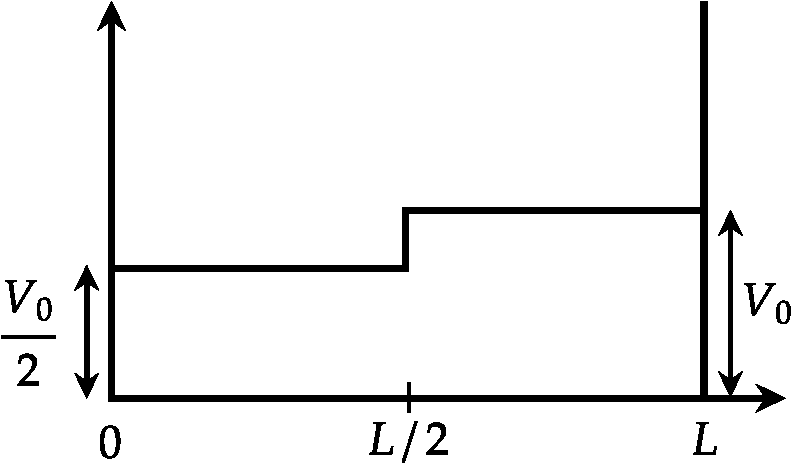
\includegraphics[height=3cm,width=5cm]{diagram-20210921(2)-crop(2)}
	\end{figure}
	$\text { The first-order correction to the ground state energy of the particle is }$
	\exyear{NET DEC 2011}
\end{minipage}
\begin{tasks}(4)
	\task[\textbf{A.}] $\frac{V_{0}}{2}$
	\task[\textbf{B.}]$\frac{3 V_{0}}{4}$
	\task[\textbf{C.}]$\frac{V_{0}}{4}$
	\task[\textbf{D.}] $\frac{3 V_{0}}{2}$
\end{tasks}
\begin{minipage}{\textwidth}
	\item Consider a two-dimensional infinite square well
	$$
	V(x, y)=\left\{\begin{array}{ll}
	0, & 0<x<a, \\
	\infty, & \text { otherwise }
	\end{array} \quad 0<y<a\right.
	$$
	Its normalized Eigenfunctions are $\psi_{n_{x}, n_{y}}(x, y)=\frac{2}{a} \sin \left(\frac{n_{x} \pi x}{a}\right) \sin \left(\frac{n_{y} \pi y}{a}\right)$,
	where $n_{x}, n_{y}=1,2,3, . .$\\
	If a perturbation $H^{\prime}=\left\{\begin{array}{cc}V_{0} & 0<x<\frac{a}{2}, \quad 0<y<\frac{a}{2} \\ 0 & \text { otherwise }\end{array}\right.$ \\is applied, then the correction to the
	energy of the first excited state to order $V_{0}$ is
	\exyear{NET JUNE 2013}
\end{minipage}
\begin{tasks}(2)
	\task[\textbf{A.}] $\frac{V_{0}}{4}$
	\task[\textbf{B.}]$\frac{V_{0}}{4}\left[1 \pm \frac{64}{9 \pi^{2}}\right]$
	\task[\textbf{C.}]$\frac{V_{0}}{4}\left[1 \pm \frac{16}{9 \pi^{2}}\right]$
	\task[\textbf{D.}]$\frac{V_{0}}{4}\left[1 \pm \frac{32}{9 \pi^{2}}\right]$
\end{tasks}
\begin{minipage}{\textwidth}
	\item Two identical bosons of mass $m$ are placed in a one-dimensional potential $V(x)=\frac{1}{2} m \omega^{2} x^{2} .$ The bosons interact via a weak potential,
	$$
	V_{12}=V_{0} \exp \left[-m \Omega\left(x_{1}-x_{2}\right)^{2} / 4 \hbar\right]
	$$
	where $x_{1}$ and $x_{2}$ denote coordinates of the particles. Given that the ground state wavefunction of the harmonic oscillator is $\psi_{0}(x)=\left(\frac{m \omega}{\pi \hbar}\right)^{\frac{1}{4}} e^{-\frac{m \omega x^{2}}{2 \hbar}} .$ The ground state energy of the two-boson system, to the first order in $V_{0}$, is
	\exyear{NET JUNE 2013}
\end{minipage}
\begin{tasks}(2)
	\task[\textbf{A.}] $\hbar \omega+2 V_{0}$
	\task[\textbf{B.}]$\hbar \omega+\frac{V_{0} \Omega}{\omega}$
	\task[\textbf{C.}]$\hbar \omega+V_{0}\left(1+\frac{\Omega}{2 \omega}\right)^{-\frac{1}{2}}$
	\task[\textbf{D.}]$\hbar \omega+V_{0}\left(1+\frac{\omega}{\Omega}\right)$
\end{tasks}
\begin{minipage}{\textwidth}
	\item The bound on the ground state energy of the Hamiltonian with an attractive deltafunction potential, namely
	$$
	H=-\frac{\hbar^{2}}{2 m} \frac{d^{2}}{d x^{2}}-a \delta(x)
	$$
	using the variational principle with the trial wavefunction $\psi(x)=A \exp \left(-b x^{2}\right)$ is\\
	$\left[\text { Note }: \int_{0}^{\infty} e^{-t} t^{a} d t=\Gamma(a+1)\right]$
	\exyear{NET JUNE 2013}
\end{minipage}
\begin{tasks}(2)
	\task[\textbf{A.}] $-m a^{2} / 4 \pi \hbar^{2}$
	\task[\textbf{B.}]$-m a^{2} / 2 \pi \hbar^{2}$
	\task[\textbf{C.}]$-m a^{2} / \pi \hbar^{2}$
	\task[\textbf{D.}]$-m a^{2} / \sqrt{5} \pi \hbar^{2}$
\end{tasks}
\begin{minipage}{\textwidth}
	\item The ground state eigenfunction for the potential $V(x)=-\delta(x)$ where $\delta(x)$ is the delta function, is given by $\psi(x)=A e^{-\alpha|x|}$, where $A$ and $\alpha>0$ are constants. If a perturbation $H^{\prime}=b x^{2}$ is applied, the first order correction to the energy of the ground state will be
	\exyear{NET JUNE 2014}
\end{minipage}
\begin{tasks}(4)
	\task[\textbf{A.}] $\frac{b}{\sqrt{2} \alpha^{2}}$ 
	\task[\textbf{B.}]$\frac{b}{\alpha^{2}}$
	\task[\textbf{C.}]$\frac{2 b}{\alpha^{2}}$
	\task[\textbf{D.}]$\frac{b}{2 \alpha^{2}}$
\end{tasks}
\begin{minipage}{\textwidth}
	\item The ground state energy of the attractive delta function potential
	$$
	V(x)=-b \delta(x) \text {, }
	$$
	where $b>0$, is calculated with the variational trial function
	$$
	\psi(x)=\left\{\begin{array}{ccc}
	A \cos \frac{\pi x}{2 a}, & \text { for } & -a<x<a, \\
	0, & & \text { otherwise, }
	\end{array}\right\} \text { is }
	$$
	\exyear{NET DEC 2014}
\end{minipage}
\begin{tasks}(2)
	\task[\textbf{A.}] $-\frac{m b^{2}}{\pi^{2} \hbar^{2}}$
	\task[\textbf{B.}]$-\frac{2 m b^{2}}{\pi^{2} \hbar^{2}}$
	\task[\textbf{C.}]$-\frac{m b^{2}}{2 \pi^{2} \hbar^{2}}$
	\task[\textbf{D.}]$-\frac{m b^{2}}{4 \pi^{2} \hbar^{2}}$
\end{tasks}
\begin{minipage}{\textwidth}
	\item Consider a particle of mass $m$ in the potential $V(x)=a|x|, a>0$. The energy eigenvalues $E_{n}(n=0,1,2, \ldots .)$, in the WKB approximation, are
	\exyear{NET DEC 2014 }
\end{minipage}
\begin{tasks}(2)
	\task[\textbf{A.}] $\left[\frac{3 a \hbar \pi}{4 \sqrt{2 m}}\left(n+\frac{1}{2}\right)\right]^{1 / 3}$
	\task[\textbf{B.}]$\left[\frac{3 a \hbar \pi}{4 \sqrt{2 m}}\left(n+\frac{1}{2}\right)\right]^{2 / 3}$
	\task[\textbf{C.}]$\frac{3 a \hbar \pi}{4 \sqrt{2 m}}\left(n+\frac{1}{2}\right)$
	\task[\textbf{D.}]$\left[\frac{3 a \hbar \pi}{4 \sqrt{2 m}}\left(n+\frac{1}{2}\right)\right]^{4 / 3}$
\end{tasks}
\begin{minipage}{\textwidth}
	\item The Hamiltonian $H_{0}$ for a three-state quantum system is given by the matrix $H_{0}=\left(\begin{array}{lll}1 & 0 & 0 \\ 0 & 2 & 0 \\ 0 & 0 & 2\end{array}\right) .$ When perturbed by $H^{\prime}=\in\left(\begin{array}{lll}0 & 1 & 0 \\ 1 & 0 & 1 \\ 0 & 1 & 0\end{array}\right)$ where $\in<<1$, the resulting shift in the energy eigenvalue $E_{0}=2$ is
	\exyear{NET DEC 2014}
\end{minipage}
\begin{tasks}(4)
	\task[\textbf{A.}] $\in,-2 \in$
	\task[\textbf{B.}] $-\in, 2 \in$
	\task[\textbf{C.}]$\pm \in$
	\task[\textbf{D.}]$\pm 2 \in$
\end{tasks}
\begin{minipage}{\textwidth}
	\item A particle of mass $m$ is in a potential $V=\frac{1}{2} m \omega^{2} x^{2}$, where $\omega$ is a constant. Let $\hat{a}=\sqrt{\frac{m \omega}{2 \hbar}}\left(\hat{x}+\frac{i \hat{p}}{m \omega}\right) .$ In the Heisenberg picture $\frac{d \hat{a}}{d t}$ is given by
	\exyear{NET JUNE 2015}
\end{minipage}
\begin{tasks}(4)
	\task[\textbf{A.}] $\omega \hat{a}$
	\task[\textbf{B.}]$-i \omega \hat{a}$
	\task[\textbf{C.}]$\omega \hat{a}^{\dagger}$
	\task[\textbf{D.}]$i \omega \hat{a}^{\dagger}$
\end{tasks}
\begin{minipage}{\textwidth}
	\item A hydrogen atom is subjected to the perturbation
	$$
	V_{\text {pert }}(r)=\epsilon \cos \frac{2 r}{a_{0}}
	$$
	where $a_{0}$ is the Bohr radius. The change in the ground state energy to first order in $\in$
	\exyear{NET DEC 2015}
\end{minipage}
\begin{tasks}(4)
	\task[\textbf{A.}] $\frac{\in}{4}$
	\task[\textbf{B.}] $\frac{\in}{2}$
	\task[\textbf{C.}]$\frac{-\epsilon}{2}$
	\task[\textbf{D.}] $\frac{-\epsilon}{4}$
\end{tasks}
\begin{minipage}{\textwidth}
	\item Consider a particle of mass $m$ in a potential $V(x)=\frac{1}{2} m \omega^{2} x^{2}+g \cos k x .$ The change in the ground state energy, compared to the simple harmonic potential $\frac{1}{2} m \omega^{2} x^{2}$, to first order in $g$ is
	\exyear{NET JUNE 2016}
\end{minipage}
\begin{tasks}(2)
	\task[\textbf{A.}] $g \exp \left(-\frac{k^{2} \hbar}{2 m \omega}\right)$
	\task[\textbf{B.}]$g \exp \left(\frac{k^{2} \hbar}{2 m \omega}\right)$
	\task[\textbf{C.}]$g \exp \left(-\frac{2 k^{2} \hbar}{m \omega}\right)$
	\task[\textbf{D.}] $g \exp \left(-\frac{k^{2} \hbar}{4 m \omega}\right)$
\end{tasks}
\begin{minipage}{\textwidth}
	\item The energy levels for a particle of mass $m$ in the potential $V(x)=\alpha|x|$, determined in the $W K B$ approximation
	$$
	\sqrt{2 m} \int_{a}^{b} \sqrt{E-V(x)} d x=\left(n+\frac{1}{2}\right) \hbar \pi
	$$
	(where $a, b$ are the turning points and $n=0,1,2 \ldots$ ), are
	\exyear{NET JUNE 2016}
\end{minipage}
\begin{tasks}(2)
	\task[\textbf{A.}] $E_{n}=\left[\frac{h \pi \alpha}{4 \sqrt{m}}\left(n+\frac{1}{2}\right)\right]^{\frac{2}{3}}$
	\task[\textbf{B.}]$E_{n}=\left[\frac{3 h \pi \alpha}{4 \sqrt{2 m}}\left(n+\frac{1}{2}\right)\right]^{\frac{2}{3}}$
	\task[\textbf{C.}]$E_{n}=\left[\frac{3 h \pi \alpha}{4 \sqrt{m}}\left(n+\frac{1}{2}\right)\right]^{\frac{2}{3}}$
	\task[\textbf{D.}] $E_{n}=\left[\frac{h \pi \alpha}{4 \sqrt{2 m}}\left(n+\frac{1}{2}\right)\right]^{\frac{2}{3}}$
\end{tasks}
\begin{minipage}{\textwidth}
	\item A particle of charge $q$ in one dimension is in a simple harmonic potential with angular frequency $\omega$. It is subjected to a time- dependent electric field $E(t)=A e^{-\left(\frac{t}{\tau}\right)^{2}}$, where $A$ and $\tau$ are positive constants and $\omega \tau \gg 1$. If in the distant past $t \rightarrow-\infty$ the particle was in its ground state, the probability that it will be in the first excited state as $t \rightarrow+\infty$ is proportional to
	\exyear{NET DEC 2016}
\end{minipage}
\begin{tasks}(2)
	\task[\textbf{A.}] $e^{-\frac{1}{2}(\omega \tau)^{2}}$
	\task[\textbf{B.}]$e^{\frac{1}{2}(\omega \tau)^{2}}$
	\task[\textbf{C.}] 0
	\task[\textbf{D.}]$\frac{1}{(\omega \tau)^{2}}$
\end{tasks}
\begin{minipage}{\textwidth}
	\item A constant perturbation $H^{\prime}$ is applied to a system for time $\Delta t$ (where $H^{\prime} \Delta t<<\hbar$ ) leading to a transition from a state with energy $E_{i}$ to another with energy $E_{f}$. If the time of application is doubled, the probability of transition will be
	\exyear{NET JUNE 2017}
\end{minipage}
\begin{tasks}(2)
	\task[\textbf{A.}] Unchanged
	\task[\textbf{B.}]Doubled
	\task[\textbf{C.}]Quadrupled
	\task[\textbf{D.}]Halved
\end{tasks}
\begin{minipage}{\textwidth}
	\item The Coulomb potential $V(r)=-e^{2} / r$ of a hydrogen atom is perturbed by adding $H^{\prime}=b x^{2}$ (where $b$ is a constant) to the Hamiltonian. The first order correction to the ground state energy is
	(The ground state wavefunction is $\psi_{0}=\frac{1}{\sqrt{\pi a_{0}^{3}}} e^{-r / a_{0}}$ )
	\exyear{NET JUNE 2017}
\end{minipage}
\begin{tasks}(4)
	\task[\textbf{A.}] $2 b a_{0}^{2}$
	\task[\textbf{B.}]$b a_{0}^{2}$
	\task[\textbf{C.}]$b a_{0}^{2} / 2$
	\task[\textbf{D.}]$\sqrt{2} b a_{0}^{2}$
\end{tasks}
\begin{minipage}{\textwidth}
	\item Consider a one-dimensional infinite square well
	$$
	V(x)=\left\{\begin{array}{lll}
	0 & \text { for } & 0<x<a \\
	\infty & & \text { otherwise }
	\end{array}\right.
	$$
	If a perturbation
	$$
	\Delta V(x)=\left\{\begin{array}{lc}
	V_{0} & \text { for } 0<x<a / 3 \\
	0 & \text { otherwise }
	\end{array}\right.
	$$
	is applied, then the correction to the energy of the first excited state, to first order in $\Delta V$, is nearest to
	\exyear{NET DEC 2017}
\end{minipage}
\begin{tasks}(4)
	\task[\textbf{A.}] $V_{0}$
	\task[\textbf{B.}]$0.16 V_{0}$
	\task[\textbf{C.}]$0.2 V_{0}$
	\task[\textbf{D.}]$0.33 V_{0}$
\end{tasks}
 \end{enumerate}
 
 \colorlet{ocre1}{ocre!70!}
 \colorlet{ocrel}{ocre!30!}
 \setlength\arrayrulewidth{1pt}
 \begin{table}[H]
 	\centering
 	\arrayrulecolor{ocre}
 	
 	\begin{tabular}{|p{1.5cm}|p{1.5cm}||p{1.5cm}|p{1.5cm}|}
 		\hline
 		\multicolumn{4}{|c|}{\textbf{Answer key}}\\\hline\hline
 		\rowcolor{ocrel}Q.No.&Answer&Q.No.&Answer\\\hline
 		1&\textbf{a}&2&\textbf{d}\\\hline
 		3&\textbf{a}&4&\textbf{b}\\\hline
 		5&\textbf{b}&6&\textbf{c}\\\hline
 		7&\textbf{c}&8&\textbf{d}\\\hline
 		9&\textbf{b}&10&\textbf{b}\\\hline
 		11&\textbf{none}&12&\textbf{b}\\\hline
 		13&\textbf{d}&14&\textbf{d}\\\hline
 		15&\textbf{b}&16&\textbf{a}\\\hline
 		17&\textbf{c}&18&\textbf{b}\\\hline
 		19&\textbf{d}&&\\\hline
 	\end{tabular}
 \end{table}




  \newpage
  \begin{abox}
  	Practice set 2
  	\end{abox}
  \begin{enumerate}
  	\begin{minipage}{\textwidth}
  	\item A particle of mass $m$ is confined in an infinite potential well:
  	$$
  	V(x)= \begin{cases}0, & \text { if } 0<x<L \\ \infty, & \text { otherwise. }\end{cases}
  	$$
  	It is subjected to a perturbing potential $V_{p}(x)=V_{o} \sin \left(\frac{2 \pi x}{L}\right)$ within the well. Let $E^{(1)}$ and $E^{(2)}$ be corrections to the ground state energy in the first and second order in $V_{0}$, respectively. Which of the following are true?
  	\exyear{GATE 2010}
  	\begin{figure}[H]
  		\centering
  		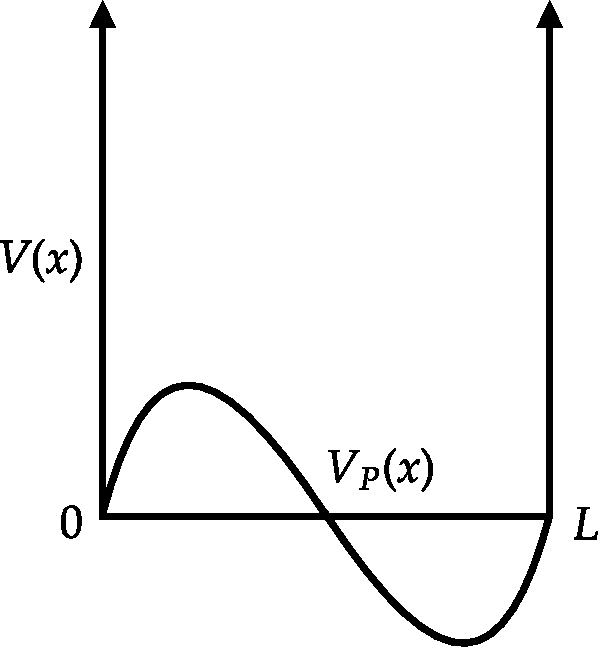
\includegraphics[height=4cm,width=5cm]{gate 2010}
  	\end{figure}
  \end{minipage}
  \begin{tasks}(2)
  	\task[\textbf{A.}]$E^{(1)}=0 ; E^{(2)}<0$
  	\task[\textbf{B.}]$E^{(1)}>0 ; E^{(2)}=0$
  	\task[\textbf{C.}]$E^{(1)}=0 ; E^{(2)}$ depends on the sign of $V_{0}$
  	\task[\textbf{D.}]$E^{(1)}<0 ; E^{(2)}<0$
  \end{tasks}
\begin{minipage}{\textwidth}
	\item The normalized eigenstates of a particle in a one-dimensional potential well
	$$
	V(x)= \begin{cases}0 & \text { if } 0 \leq x \leq a \\ \infty & \text { otherwise }\end{cases}
	$$
	are given by $\psi_{n}(x)=\sqrt{\frac{2}{a}} \sin \left(\frac{n \pi x}{a}\right)$, where $n=1,2,3, \ldots . .$
	The particle is subjected to a perturbation
	$$
	V^{\prime}(x)= \begin{cases}V_{0} \cos \left(\frac{\pi x}{a}\right), & \text { for } 0 \leq x \leq \frac{a}{2} \\ 0, & \text { otherwise }\end{cases}
	$$
	The shift in the ground state energy due to the perturbation, in the first order perturbation theory,
	\exyear{GATE 2011}
\end{minipage}
\begin{tasks}(4)
	\task[\textbf{A.}] $\frac{2 V_{o}}{3 \pi}$
	\task[\textbf{B.}]$\frac{V_{o}}{3 \pi}$
	\task[\textbf{C.}]$-\frac{V_{o}}{3 \pi}$
	\task[\textbf{D.}]$-\frac{2 V_{o}}{3 \pi}$
\end{tasks}
\begin{minipage}{\textwidth}
	\item Consider a system in the unperturbed state described by the Hamiltonian, $H_{0}=\left(\begin{array}{ll}1 & 0 \\ 0 & 1\end{array}\right)$. The system is subjected to a perturbation of the form $H^{\prime}=\left(\begin{array}{ll}\delta & \delta \\ \delta & \delta\end{array}\right)$, where $\delta \ll<1$. The energy eigenvalues of the perturbed system using the first order perturbation approximation are
	\exyear{GATE 2012}
\end{minipage}
\begin{tasks}(2)
	\task[\textbf{A.}]1 and $(1+2 \delta)$
	\task[\textbf{B.}]$(1+\delta)$ and $(1-\delta)$
	\task[\textbf{C.}]$(1+2 \delta)$ and $(1-2 \delta)$
	\task[\textbf{D.}]$(1+\delta)$ and $(1-2 \delta)$
\end{tasks}
\textbf{\text { Common data questions } 4 \text { and } 5}\\
$\begin{aligned}
&\text { To the given unperturbed Hamiltonian }\left[\begin{array}{ccc}
5 & 2 & 0 \\
2 & 5 & 0 \\
0 & 0 & 2
\end{array}\right] \\
&\text { we add a small perturbation given by } \varepsilon\left[\begin{array}{ccc}
1 & 1 & 1 \\
1 & 1 & -1 \\
1 & -1 & 1
\end{array}\right] \text { where } \varepsilon \text { is small quantity. }
\end{aligned}$\\
\begin{minipage}{\textwidth}
	\item $\text { The ground state eigenvector of the unperturbed Hamiltonian is }$
	\exyear{GATE 2013}
\end{minipage}
\begin{tasks}(2)
	\task[\textbf{A.}] $(1 / \sqrt{2}, 1 \sqrt{2}, 0)$
	\task[\textbf{B.}]$(1 / \sqrt{2},-1 / \sqrt{2}, 0)$
	\task[\textbf{C.}] $(0,0,1)$
	\task[\textbf{D.}]$(1,0,0)$
\end{tasks}
\begin{minipage}{\textwidth}
	\item A pair of eigenvalues of the perturbed Hamiltonian, using first order perturbation theory, is
	\exyear{GATE 2013}
\end{minipage}
\begin{tasks}(2)
	\task[\textbf{A.}]$3+2 \varepsilon, 7+2 \varepsilon$
	\task[\textbf{B.}]$3+2 \varepsilon,+2+\varepsilon$
	\task[\textbf{C.}]$3,7+2 \varepsilon$
	\task[\textbf{D.}]$3,2+2 \varepsilon$
\end{tasks}
\begin{minipage}{\textwidth}
	\item A particle is confined to a one dimensional potential box, with the potential
	$$
	V(x)= \begin{cases}0, & 0<x<a \\ \infty, & \text { otherwise }\end{cases}
	$$
	If particle is subjected to a perturbation within the box. $W=\beta x$. Where $\beta$ is small constant, the first order correction to the ground state energy is
	\exyear{GATE 2014}
\end{minipage}
\begin{tasks}(4)
	\task[\textbf{A.}] 0
	\task[\textbf{B.}]$a \beta / 4$
	\task[\textbf{C.}]$a \beta / 2$
	\task[\textbf{D.}] $a \beta$
\end{tasks}
\begin{minipage}{\textwidth}
	\item A particle is confined in a box of length $L$ as shown in the figure. If the potential $V_{0}$ is treated as a perturbation, including the first order correction, the ground state energy is
	\exyear{GATE 2015}
	\begin{figure}[H]
		\centering
		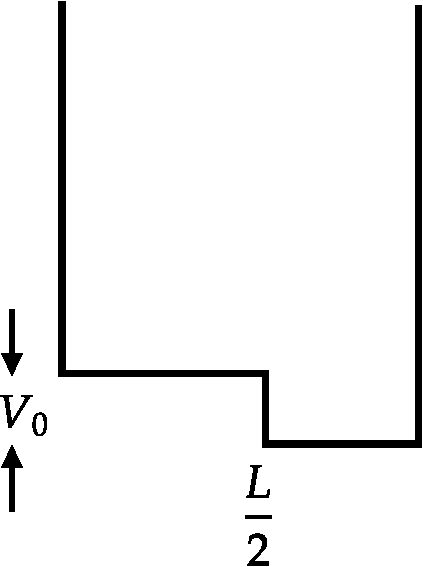
\includegraphics[height=3cm,width=3cm]{diagram-20210824(7)-crop}
	\end{figure}
\end{minipage}
\begin{tasks}(2)
	\task[\textbf{A.}] $E=\frac{\hbar^{2} \pi^{2}}{2 m L^{2}}+V_{0}$
	\task[\textbf{B.}]$E=\frac{\hbar^{2} \pi^{2}}{2 m L^{2}}-\frac{V_{0}}{2}$
	\task[\textbf{C.}] $E=\frac{\hbar^{2} \pi^{2}}{2 m L^{2}}+\frac{V_{0}}{4}$
	\task[\textbf{D.}]$E=\frac{\hbar^{2} \pi^{2}}{2 m L^{2}}+\frac{V_{0}}{2}$
\end{tasks}
\begin{minipage}{\textwidth}
	\item A one dimensional simple harmonic oscillator with Hamiltonian $H_{0}=\frac{p^{2}}{2 m}+\frac{1}{2} k x^{2}$ is subjected to a small perturbation, $H_{1}=\alpha x+\beta x^{3}+\gamma x^{4}$. The first order correction to the ground state energy is dependent on
	\exyear{GATE 2017}
\end{minipage}
\begin{tasks}(4)
	\task[\textbf{A.}] only $\beta$
	\task[\textbf{B.}]$\alpha$ and $\gamma$
	\task[\textbf{C.}]$\alpha$ and $\beta$
	\task[\textbf{D.}]only $\gamma$
\end{tasks}
  \end{enumerate}
\colorlet{ocre1}{ocre!70!}
\colorlet{ocrel}{ocre!30!}
\setlength\arrayrulewidth{1pt}
\begin{table}[H]
	\centering
	\arrayrulecolor{ocre}
	
	\begin{tabular}{|p{1.5cm}|p{1.5cm}||p{1.5cm}|p{1.5cm}|}
		\hline
		\multicolumn{4}{|c|}{\textbf{Answer key}}\\\hline\hline
		\rowcolor{ocrel}Q.No.&Answer&Q.No.&Answer\\\hline
		1&\textbf{a}&2&\textbf{a}\\\hline
		3&\textbf{a}&4&\textbf{c}\\\hline
		5&\textbf{c}&6&\textbf{c}\\\hline
		7&\textbf{d}&8&\textbf{d}\\\hline
	\end{tabular}
\end{table}
\newpage
\begin{abox}
	Practice set 3
	\end{abox}
 \begin{enumerate}
 		\begin{minipage}{\textwidth}
 		\item A one dimensional infinite potential box is defined by, $V(x)=\left\{\begin{array}{ll}0, & 0<x<a \\ \infty, & \text { otherwise }\end{array}\right.$. It is perturbed by potential $\frac{\alpha V_{0} x^{2}}{a^{2}}$, then find the first order energy correction in $n^{t h}$ state of the system.
 	\end{minipage}
 	\begin{answer}
 	$$E_{n}^{1}=\left\langle\phi_{n}|W| \phi_{n}\right\rangle, \text { where }\left|\phi_{n}\right\rangle=\sqrt{\frac{2}{a}} \sin \frac{n \pi x}{a}$$
 	\begin{align*}
 		&E_{n}^{1}=V_{0} \frac{2}{a} \int_{0}^{a} \frac{x^{2}}{a^{2}} \sin ^{2} \frac{n \pi x}{a} d x=V_{0} \frac{1}{a} \int_{0}^{a} \frac{x^{2}}{a^{2}}\left(1-\cos \frac{2 n \pi x}{a}\right) d x=V_{0}\left(\frac{1}{3}-\frac{1}{2 n^{2} \pi^{2}}\right) \\
 		&E_{n}=\frac{n^{2} \pi^{2}}{2 m a^{2}}+\alpha V_{0}\left(\frac{1}{3}-\frac{1}{2 n^{2} \pi^{2}}\right)
 	\end{align*}	
 	\end{answer}
 	\begin{minipage}{\textwidth}
 	\item A one dimensional infinite potential box is defined as, $V(x)= \begin{cases}0, & -\frac{L}{2}<x<\frac{L}{2} . \text { It } \\ \infty, & \text { otherwise }\end{cases}$ is perturbed with potential $H_{p}=V_{0} \exp \left(-\frac{x^{2}}{a^{2}}\right) .$ Find the first order energy correction in ground state with momentum $\frac{\pi \hbar}{L}$ by assuming $\frac{a}{L}<<1$.
 \end{minipage}
 \begin{answer}
  $\left|\phi_{1}\right\rangle=\sqrt{\frac{1}{L}} \exp \frac{i \pi x}{L}, \text { because momentum is } \frac{\pi \hbar}{L}$\\
  \begin{align*}
  	&E_{1}^{1}=\left\langle\phi_{1}|W| \phi_{1}\right\rangle=\frac{V_{0}}{L} \int_{-L / 2}^{L / 2} \exp \left(-\frac{x^{2}}{a^{2}}\right) d x, \text { if } \frac{a}{L}<<1 \text { then } \\
  	&E_{1}^{1}=\frac{V_{0}}{L} \int_{-\infty}^{\infty} \exp \left(-\frac{x^{2}}{a^{2}}\right) d x=\frac{\sqrt{\pi} V_{0} a}{L} .
  \end{align*}
 \end{answer}
	\begin{minipage}{\textwidth}
	\item A one dimensional infinite potential box is defined as, $V(x)= \begin{cases}0, & -\frac{a}{2}<x<\frac{a}{2} . \text { It is } \\ \infty, & \text { otherwise }\end{cases}$ perturbed with potential $H_{p}=V_{0} a \delta(x)$. Find the $E_{n}^{2}$.i.e., second order correction in ground state.
\end{minipage}
\begin{answer}
	$E_{n}^{2}=\sum_{m \neq n} \frac{\left|\left\langle\phi_{m}|W| \phi_{n}\right\rangle\right|^{2}}{E_{n}-E_{m}}$\\
	If $n$ is even, then $\left\langle\phi_{m}|W| \phi_{n}\right\rangle=0$\\
	If $m$ is even, then $\left\langle\phi_{m}|W| \phi_{n}\right\rangle=0$\\
	If $m$ and $n$ odd, then $\left\langle\phi_{m}|W| \phi_{n}\right\rangle=V_{0} a\left(\frac{2}{a}\right)\int_{-a / 2}^{a / 2} \cos \frac{m \pi x}{a} \cos \frac{n \pi x}{a} \delta(x) d x=2 V_{0}$
	$$
	E_{n}^{2}=\sum_{m \neq n} \frac{\left|\left\langle\phi_{m}|W| \phi_{n}\right\rangle\right|^{2}}{E_{n}-E_{m}}=\sum_{m=1,3,5} \frac{4 V_{0}^{2}}{\left(n^{2}-m^{2}\right) E_{0}}, \text { where } E_{0}=\frac{\pi^{2} \hbar^{2}}{2 m a^{2}}
	$$
\end{answer}
	\begin{minipage}{\textwidth}
	\item A one dimensional harmonic oscillator with potential, $V(x)=\frac{1}{2} m \omega^{2} x^{2}$ is given, then\\
	(a) if H.O potential is perturbed with perturbation $H_{p}=\lambda X^{4}$, then find the first order energy correction in $n^{\text {th }}$ state of the system.\\
	(b) if H.O Perturbed with potential $V_{0} \cosh \alpha x$, then find the first order energy correction in ground state.
\end{minipage}
\begin{answer}
(a)	$E_{n}^{1}=\left\langle\phi_{n}\left|H_{p}\right| \phi_{n}\right\rangle=\left\langle\phi_{n}\left|\lambda X^{4}\right| \phi_{n}\right\rangle$\\
	$=\lambda\left(\frac{\hbar}{2 m \omega}\right)^{2}\left\langle\left(a+a^{\dagger}\right)^{4}\right\rangle=\left(\frac{\hbar}{2 m \omega}\right)^{2}\left[6 n^{2}+6 n+3\right]$\\
	(b)$ E_{0}^{1}=\left\langle\phi_{0}|W| \phi_{0}\right\rangle, \text { where }\left|\phi_{0}\right\rangle=\left(\frac{m \omega}{\pi \hbar}\right)^{1 / 4} \exp \left(-\frac{m \omega x^{2}}{2 \hbar}\right) \text {. }$\\
	\begin{align*}
		&=\left(\frac{m \omega}{\pi \hbar}\right)^{1 / 2} V_{0} \int_{-\infty}^{\infty} \exp \left(-\frac{m \omega x^{2}}{\hbar}\right) \cosh \alpha x d x \\
		&=V_{0}\left(\frac{m \omega}{\pi \hbar}\right)^{1 / 2} \int_{-\infty}^{\infty} \exp \left(-\frac{m \omega x^{2}}{\hbar}\right) \frac{\left(e^{\alpha x}+e^{-\alpha x}\right)}{2} d x \\
		&=\frac{V_{0}}{2}\left(\frac{m \omega}{\pi \hbar}\right)^{1 / 2}\left(\int_{-\infty}^{\infty} e^{-\frac{m \omega}{\hbar}\left(x-\frac{\hbar}{2 m \omega}\right)^{2}}\left(e^{\frac{\hbar}{4 m \omega}}\right) d x+\int_{-\infty}^{\infty} e^{-\frac{m \omega}{\hbar}\left(x+\frac{\hbar}{2 m \omega}\right)^{2}} \cdot\left(-e^{\frac{\hbar}{4 m \omega}}\right) d x\right) \\
		&=\frac{V_{0}}{2}\left(\exp \frac{\hbar}{4 m \omega}+\exp \frac{\hbar}{4 m \omega}\right)=V_{0} \exp \frac{\hbar}{4 m \omega}
	\end{align*}
\end{answer}
	\begin{minipage}{\textwidth}
	\item
	One dimensional potential is given by, $V(x)=\left\{\begin{array}{ll}\infty, & x<0 \\ \frac{1}{2} m \omega^{2} x^{2}, & x \geq 0\end{array} .\right.$ It is perturbed by potential\\
	(a) $H_{p}=\lambda V_{0}$, then find the first order correction in energy for ground state .\\
	(b) $H_{p}=\lambda V_{0} \delta\left(x-\sqrt{\frac{\hbar}{m \omega}}\right)$, find the first order correction in energy for ground state .\\
	(c) $H_{p}=\lambda X$\\
	(d) $H_{p}=\lambda X^{2}$\\
\end{minipage}
\begin{answer}
	$\text { For given system first excited state } n=1$\\
	$\left|\phi_{1}\right\rangle= \begin{cases}0, & \text { if } \quad x<0 \\ 2\left(\frac{m \omega}{\pi \hbar}\right)^{1 / 4}\left(\frac{m \omega}{\hbar}\right)^{1 / 2} x \exp \left(-\frac{m \omega x^{2}}{2 \hbar}\right) ; & 0<x<\infty\end{cases}$\\
(a)	$E_{0}^{\prime}=V_{0}(4 \pi)\left(\frac{m \omega}{\pi \hbar}\right)^{3 / 2 } \int_{0}^{\infty} x^2e^{-\frac{m \omega x^{2}}{\hbar}} d x=V_{0}(4 \pi)\left(\frac{m \omega}{\pi \hbar}\right)^{3 / 2} \frac{1}{2}\left(\frac{\hbar}{m \omega}\right)^{3 / 2} \frac{1}{2} \sqrt{\pi}=V_{0}$\\\\
(b)$H_{p}=\lambda V_{0} \delta\left(x-\sqrt{\frac{\hbar}{m \omega}}\right)$
\begin{align*}
E_{0}^{\prime}&=V_{0} \cdot 4 \pi\left(\frac{m \omega}{\pi \hbar}\right)^{3 / 2} \int_{0}^{\infty} x^{2} e^{-\frac{m \omega x^{2}}{\hbar}} \int\left(x-\sqrt{\frac{\hbar}{m \omega}}\right) d x\\
&=\left(4 \pi V_{0}\right)\left(\frac{m \omega}{\pi \hbar}\right)^{3 / 2}\left(\sqrt{\frac{\hbar}{m \omega}}\right)^{2} e^{-\frac{m \omega}{\hbar} \cdot\left(\frac{m \omega}{\hbar}\right)}\\
&=\frac{4 \pi V_{0}}{\pi^{3 / 2}}\left(\frac{m \omega}{\hbar}\right)^{1 / 2} e^{-1}=4 V_{0}\left(\frac{m \omega}{\hbar}\right)^{1 / 2} e^{-1}=4 V_{0} \sqrt{\frac{m \omega}{\pi \hbar}} e^{-1}
\end{align*}
$\text { (d) } H_{p}=\lambda x^{2}$
\begin{align*}
E_{0}^{\prime}&=4 \pi\left(\frac{m \omega}{\pi \hbar}\right)^{3 / 2} \int_{0}^{\infty} x^{3} e^{-\frac{m \omega x^{2}}{\hbar}} d x\\
&=4 \pi\left(\frac{m \omega}{\pi \hbar}\right)^{3 / 2} \frac{1}{2}\left(\frac{\hbar}{m \omega}\right)^{2} \times 1=2 \times \sqrt{\frac{\hbar}{\pi m \omega}}
\end{align*}
$\text { (d) } H_{p}=\lambda x^{2}$\\
\begin{align*}
E_{0}^{\prime}&=4 \pi\left(\frac{m \omega}{\pi \hbar}\right)^{3 / 2} \int_{0}^{\infty} x^{4} e^{-\frac{m \omega x^{2}}{h}} d x\\
&=4 \pi\left(\frac{m \omega}{\pi \hbar}\right)^{3 / 2}\left(\frac{\hbar}{m \omega}\right)^{5 / 2} \times \frac{1}{2} \times \frac{3}{4} \sqrt{\pi}=\frac{3}{2}\left(\frac{\hbar}{m \omega}\right)
\end{align*}
\end{answer}
	\begin{minipage}{\textwidth}
	\item $\text { If Harmonic Potential is given by } V=\frac{1}{2} m \omega^{2} x^{2} \text { and wave function is given as }$\\
	$$
	\psi(x)= \begin{cases}A \cos \frac{\pi x}{a}, & \frac{-a}{2}<x<\frac{a}{2} \\ 0 & , \quad \text { otherwise }\end{cases}
	$$
	then find the ground state energy.
\end{minipage}
\begin{answer}
$\text { Since, }\langle\psi \mid \psi\rangle=1 \Rightarrow|A|=\sqrt{\frac{2}{a}}$\\
Hence, $|\psi\rangle=\sqrt{\frac{2}{a}} \cos \left(\frac{\pi x}{a}\right), \frac{-a}{2}<x<\frac{a}{2}$\\
And also, average kinetic energy, $\langle T\rangle=\frac{\pi^{2} \hbar^{2}}{2 m a^{2}}$	\\
\begin{align*}
\langle V\rangle&=\frac{1}{2} m \omega^{2} \int_{-a / 2}^{a / 2}\left(\sqrt{\frac{2}{a}}\right)^{2} x^{2} \cos ^{2}\left(\frac{\pi x}{a}\right) d x\\
&=\frac{1}{-2} \frac{m \omega^{2}}{a} \int_{-a / 2}^{a / 2}\left[x^{2}\left(1+\cos \frac{2 \pi x}{a}\right)\right] d x\\
&=\frac{m \omega^{2}}{2 a}\left[\frac{1}{3}\left(x^{3}\right)_{-a / 2}^{a / 2}+x^{2} \frac{a}{2 \pi} \sin \left(\frac{2 \pi x}{a}\right)-\frac{a}{\pi}\left\{x\left(-\frac{a}{2 \pi}\right) \cos \frac{2 \pi x}{a}+\left(\frac{a}{2 \pi}\right)^{2} \sin \frac{2 \pi x}{a}\right\}\right]_{-a / 2}^{a / 2}\\
\langle V\rangle&=\frac{m \omega^{2}}{2 a}\left[\frac{a^{3}}{12}-\frac{a^{3}}{2 \pi^{2}}\right]=\frac{m \omega^{2} a^{2}}{4}\left(\frac{1}{6}-\frac{1}{\pi^{2}}\right)\\
\text { Hence, }\langle E\rangle&=\langle T\rangle+\langle V\rangle=\left(\frac{\pi^{2} \hbar^{2}}{2 m a^{2}}\right)+\frac{m \omega^{2} a^{2}}{4}\left(\frac{1}{6}-\frac{1}{\pi^{2}}\right)\\
&\text { For minimum energy, } \frac{d\langle E\rangle}{d a}=0\\
&\Rightarrow \frac{\pi^{2} \hbar^{2}}{2 m}\left(-\frac{2}{a^{3}}\right)+\frac{m \omega^{2} a}{2}\left(\frac{1}{6}-\frac{1}{\pi^{2}}\right)=0 \Rightarrow a=\left[\frac{2 \pi^{2} \hbar^{2}}{m^{2} \omega^{2}} \times\left(\frac{6 \pi^{2}}{\pi^{2}-6}\right)\right]^{1 / 4} \\
\therefore\langle E\rangle&=\hbar \omega\left(\frac{\pi^{2}}{12}-\frac{1^{-}}{2}\right)^{1 / 2}
\end{align*}
\end{answer}
	\begin{minipage}{\textwidth}
	\item Using the trial wave-function, $\psi=e^{-a r}$, find the ground state energy of $3-D$ harmonic oscillator with potential $V=\frac{1}{2} m \omega^{2} r^{2}$.
\end{minipage}
\begin{answer}
	$V=\frac{1}{2} m \omega^{2} r^{2}$\\
	\begin{align*}
		&\text { Trial wave function, } \psi=e^{-u r} \\
		&\because \quad \text { Normalising, } \psi=|A|^{2} \cdot 4 \pi \int_{0}^{\infty} r^{2} e^{-2 \alpha r} d r=1 \Rightarrow|A|=\sqrt{\frac{\alpha^{3}}{\pi}}
	\end{align*}
	$\langle T\rangle=-\frac{\hbar^{2}}{2 m} 4 \pi \int_{0}^{\infty} \psi^{\cdot}\left(\frac{d^{2}}{d r^{2}}+\frac{2}{r}\right) \psi r^{2} d r, \text { where } \psi=\sqrt{\frac{\alpha^{3}}{\pi}} e^{-\alpha r}$\\
	\begin{align*}
		&\langle T\rangle=-\frac{\hbar^{2}}{2 m}\left(\frac{\alpha^{3}}{\pi}\right) 4 \pi \int_{0}^{\infty} e^{-\alpha r}\left(\alpha^{2}-\frac{2 \alpha}{r}\right) e^{-\alpha r} r^{2} d r \\
		&\langle T\rangle=-\frac{\hbar^{2}}{2 m}\left(\frac{\alpha^{3}}{\pi}\right) 4 \pi\left(\alpha^{2} \int_{0}^{\infty} e^{-2 \alpha r} r^{2} d r-2 \alpha \int_{0}^{\infty} e^{-2 \alpha r} r d r\right) \\
		&=\frac{-\hbar^{2} \alpha^{3}}{2 m \pi} 4 \pi\left[\alpha^{2}\left(\frac{1}{2 \alpha}\right)^{3}\left\lfloor 2-2 \alpha\left(\frac{1}{2 \alpha}\right)^{2}\right]=\frac{-\hbar^{2} \alpha^{3}}{2 m \pi} 4 \pi\left[\frac{1}{4 \alpha}-\frac{1}{2 \alpha}\right]\right.\\
		&\langle T\rangle=\frac{\hbar^{2} \alpha^{2}}{2 m} \\
		&\langle V\rangle=\frac{\alpha^{3}}{\pi} \times \frac{1}{2} m \omega^{2} \times 4 \pi \int_{0}^{\infty} r^{2} r^{2} e^{-2 \alpha r} d r=\frac{3 \omega^{2} m}{2 \alpha^{2}} \\
		&\therefore\langle E\rangle=\frac{\hbar^{2} \alpha^{2}}{2 m}+\frac{3 \omega^{2} m}{2 \alpha^{2}}\\
		&\frac{d\langle E\rangle}{d \alpha}=0 \Rightarrow \frac{\hbar^{2} \alpha}{m}-\frac{3 \omega^{2} m}{\alpha^{3}}=0 \Rightarrow \alpha=\left(\frac{3 m^{2} \omega^{2}}{\hbar^{2}}\right)^{1 / 4} \\
		&\langle E\rangle=\frac{\hbar^{2}}{2 m}\left(\frac{3 m^{2} \omega^{2}}{\hbar^{2}}\right)^{1 / 2}+\frac{3 \omega^{2} m}{2}\left(\frac{\hbar^{2}}{3 m^{2} \omega^{2}}\right)^{1 / 2} \\
		&=\frac{1}{2}\left(3 \hbar^{2} \omega^{2}\right)^{1 / 2}+\frac{1}{2}\left(3 \hbar^{2} \omega^{2}\right)^{1 / 2} \Rightarrow\langle E\rangle=\sqrt{3} \hbar \omega
	\end{align*}
\end{answer}
	\begin{minipage}{\textwidth}
	\item A particle in one dimension moves under the influence of a potential $V(x)=a x^{6}$, where $a$ is a real constant. For large $n$ the quantized energy level $E_{n}$ depends on $n$ as $E_{n}=n^{\alpha}$ then find the value of $\alpha$.
\end{minipage}
\begin{answer}$\left. \right. $\\
	\begin{minipage}{0.5\textwidth}
	$V(x)=a x^{6} \text { and } E=\frac{p^{2}}{2 m}+a x^{6}$\\
	According to Bohr Somerfield theory $\oint p d x=n h, n=1,2 \ldots$\\\\
	$
	\oint \sqrt{2 m\left(E-a x^{6}\right)} d x=n h, n=1,2 \ldots
	$
	\end{minipage}
	 \begin{minipage}{0.5\textwidth}
	 \begin{figure}[H]
	 	\centering
	 	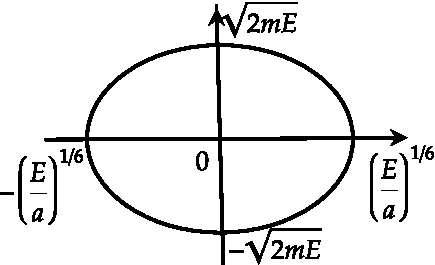
\includegraphics[height=3cm,width=5cm]{diagram-20220205-20220205160131-crop}
	 \end{figure}
	 \end{minipage}
	 $$\text { 4. } \int_{0}^{\left(\frac{E}{a}\right)} \sqrt{2 m\left(E-a x^{6}\right)} d x=n h \Rightarrow 4 \sqrt{2 m E} \int_{0}^{\frac{E}{a}} \int_{1 / 6}^{1 / 6} \sqrt{\left(1-\frac{a x^{6}}{E}\right)} d x=n h, n=1,2 \ldots$$
	 \begin{align*}
	 	&\text { Put }\left(\frac{a}{E}\right)^{1 / 6} x=t \text { then } d x=d t\left(\frac{E}{a}\right)^{\frac{1}{6}} \Rightarrow 4 \sqrt{2 m E} \cdot\left(\frac{E}{a}\right)^{1 / 6} \int_{0}^{1} \sqrt{\left(1-t^{6}\right)} d t=n h \\
	 	&\Rightarrow E^{\frac{1}{2}+\frac{1}{6}} \propto n \Rightarrow E^{\frac{4}{6}} \propto n \Rightarrow E \propto n^{\frac{3}{2}} \text { so value of } \alpha=\frac{3}{2}
	 \end{align*}
\end{answer}
	\begin{minipage}{\textwidth}
	\item A particle of mass $m$ interacts with potential $V(x)=\left\{\begin{array}{l}\infty, x \leq 0 \\ \lambda x, x \geq 0\end{array} .\right.$ Using the WKB approximation Find the energy of bound state system.
\end{minipage}
\begin{answer}
$\text { For bound state system } E>0 \text { where } E=\frac{p^{2}}{2 m}+\lambda x \Rightarrow p=\sqrt{2 m(E-\lambda x)}$\\
The two turning points are given by $x_{1}=0$ and $x_{2}=\frac{E}{\lambda}$\\
In the given potential one boundary is rigid and another is smooth so according to WKB
Approximation Bound state is given by $\int_{x_{1}}^{x_{2}} p d x=\left(n+\frac{3}{4}\right) \pi \hbar$, where $n=0,1,2$\\
\begin{minipage}{0.5\textwidth}
$\sqrt{2 m E} \int_{0}^{\frac{E}{\lambda}} \sqrt{1-\left(\frac{\lambda}{E}\right)} x d x=\left(n+\frac{3}{4}\right) \pi \hbar$ where $n=0,1,2$ \\
$\frac{\lambda}{E} x=t \Rightarrow d x=\frac{E}{\lambda} d t$\\
\end{minipage}
\begin{minipage}{0.5\textwidth}
\begin{figure}[H]
	\centering
	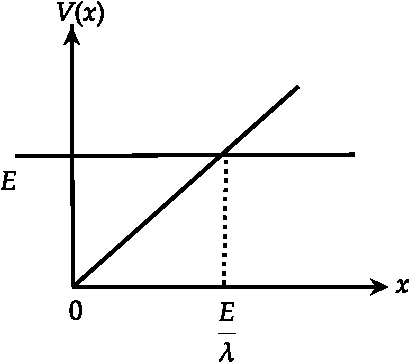
\includegraphics[height=3cm,width=5cm]{diagram-20220205(1)-20220205162522-crop}
\end{figure}
\end{minipage}
So the integration is given by $\sqrt{2 m E} \cdot \frac{E}{\lambda} \int_{0}^{1} \sqrt{1-t} d t=(n+3 / 4) \pi \hbar, n=0 ; 1,2 \ldots$ To find $I=\int_{0}^{1} \sqrt{1-t} d t$\\
\begin{align*}
	&\text { put } 1-t=y-d t=d y \text { so } I=-\int_{1}^{0} \sqrt{y} d y \quad \Rightarrow \int_{0}^{1} y^{1 / 2} d y=\frac{\left(y^{3 / 2}\right)_{0}^{1}}{3 / 2}=\frac{2}{3} \\
	&\sqrt{2 m E} \cdot \frac{E}{\lambda} \int_{0}^{1} \sqrt{1-t} d t=\sqrt{2 m E} \cdot \frac{E}{\lambda} \times \frac{2}{3}=\left(n+\frac{3}{4}\right) \pi \hbar \quad \text { where } n=0,1,2 \ldots \\
	&=E^{3 / 2} \cdot 2 \frac{\sqrt{2 m}}{3 \lambda}=\left(n+\frac{3}{4}\right) \pi \hbar \Rightarrow E=\left[\frac{3 \hbar \pi \lambda}{2 \sqrt{2 m}}(n+3 / 4)\right]^{\frac{2}{3}} n=0,1,2 \ldots . .
\end{align*}	
\end{answer}
 \end{enumerate}
 
 
 
 
 
 
 
 
 
 
 
 
 
 
 
 
 
 
 
 
 
 
 
 
 
 
 
 
 
 
 
 
 
 
 
 
 
 
 
 
 
 
 
 
 
 
 
 
 
 
 
 
 
 
 
 
 
 
 
 
 
 
